%definira klasu dokumenta 
\documentclass[12pt]{report} 

%prostor izmedu naredbi \documentclass i \begin{document} se zove uvod. U njemu se nalaze naredbe koje se odnose na cijeli dokument

%osnovni LaTex ne može riješiti sve probleme, pa se koriste različiti paketi koji olakšavaju izradu željenog dokumenta
\usepackage[croatian]{babel} 
\usepackage{amssymb}
\usepackage{amsmath}
\usepackage{txfonts}
\usepackage{mathdots}
\usepackage{titlesec}
\usepackage{array}
\usepackage{lastpage}
\usepackage{etoolbox}
\usepackage{tabularray}
\usepackage{color, colortbl}
\usepackage{adjustbox}
\usepackage{geometry}
\usepackage[classicReIm]{kpfonts}
\usepackage{hyperref}
\usepackage{fancyhdr}

\usepackage{float}
\usepackage{setspace}
\restylefloat{table}


\patchcmd{\chapter}{\thispagestyle{plain}}{\thispagestyle{fancy}}{}{} %redefiniranje stila stranice u paketu fancyhdr

%oblik naslova poglavlja
\titleformat{\chapter}{\normalfont\huge\bfseries}{\thechapter.}{20pt}{\Huge}
\titlespacing{\chapter}{0pt}{0pt}{40pt}


\linespread{1.3} %razmak između redaka

\geometry{a4paper, left=1in, top=1in,}  %oblik stranice

\hypersetup{ colorlinks, citecolor=black, filecolor=black, linkcolor=black,	urlcolor=black }   %izgled poveznice


%prored smanjen između redaka u nabrajanjima i popisima
\newenvironment{packed_enum}{
	\begin{enumerate}
		\setlength{\itemsep}{0pt}
		\setlength{\parskip}{0pt}
		\setlength{\parsep}{0pt}
	}{\end{enumerate}}

\newenvironment{packed_item}{
	\begin{itemize}
		\setlength{\itemsep}{0pt}
		\setlength{\parskip}{0pt}
		\setlength{\parsep}{0pt}
	}{\end{itemize}}




%boja za privatni i udaljeni kljuc u tablicama
\definecolor{LightBlue}{rgb}{0.9,0.9,1}
\definecolor{LightGreen}{rgb}{0.9,1,0.9}

%Promjena teksta za dugačke tablice
\DefTblrTemplate{contfoot-text}{normal}{Nastavljeno na idućoj stranici}
\SetTblrTemplate{contfoot-text}{normal}
\DefTblrTemplate{conthead-text}{normal}{(Nastavljeno)}
\SetTblrTemplate{conthead-text}{normal}
\DefTblrTemplate{middlehead,lasthead}{normal}{Nastavljeno od prethodne stranice}
\SetTblrTemplate{middlehead,lasthead}{normal}

%podesavanje zaglavlja i podnožja

\pagestyle{fancy}
\lhead{Programsko inženjerstvo}
\rhead{ConnectiNET}
\lfoot{Spajalice}
\cfoot{stranica \thepage/\pageref{LastPage}}
\rfoot{\today}
\renewcommand{\headrulewidth}{0.2pt}
\renewcommand{\footrulewidth}{0.2pt}


\begin{document} 
	
	
	
	\begin{titlepage}
		\begin{center}
			\vspace*{\stretch{1.0}} %u kombinaciji s ostalim \vspace naredbama definira razmak između redaka teksta
			\LARGE Programsko inženjerstvo\\
			\large Ak. god. 2023./2024.\\
			
			\vspace*{\stretch{3.0}}
			
			\huge ConnectiNET\\
			\Large Dokumentacija, Rev. \textit{1}\\
			
			\vspace*{\stretch{12.0}}
			\normalsize
			Grupa: \textit{Spajalice}\\
			Voditelj: \textit{Mario Mrvčić}\\
			
			
			\vspace*{\stretch{1.0}}
			Datum predaje: \textit{17. studenog 2023.}\\
	
			\vspace*{\stretch{4.0}}
			
			Nastavnik: \textit{Nikolina Frid}\\
		
		\end{center}

	
	\end{titlepage}

	
	\tableofcontents


	\chapter{Dnevnik promjena dokumentacije}
		
		\textbf{\textit{Kontinuirano osvježavanje}}\\
				
		
		\begin{longtblr}[
				label=none
			]{
				width = \textwidth, 
				colspec={|X[2]|X[13]|X[3]|X[3]|}, 
				rowhead = 1
			}
			\hline
			\textbf{Rev.}	& \textbf{Opis promjene/dodatka} & \textbf{Autori} & \textbf{Datum}\\[3pt] \hline
			0.1 & Napravljen predložak.	& * & 22.08.2013. 		\\[3pt] \hline 
			0.2	& Dopisane upute za povijest dokumentacije.\newline Dodane reference. & * & 24.08.2013. 	\\[3pt] \hline 
			0.5 & Dodan \textit{Use Case} dijagram i jedan sekvencijski dijagram, funkcionalni i nefunkcionalni zahtjevi i dodatak A & * & 25.08.2013. \\[3pt] \hline 
			0.6 & Arhitektura i dizajn sustava, algoritmi i strukture podataka & * & 26.08.2013. \\[3pt] \hline 
			0.8 & Povijest rada i trenutni status implementacije,\newline Zaključci i plan daljnjeg rada & * & 28.08.2013. \\[3pt] \hline 
			0.9 & Opisi obrazaca uporabe & * & 07.09.2013. \\[3pt] \hline 
			0.10 & Preveden uvod & * & 08.09.2013. \\[3pt] \hline 
			0.11 & Sekvencijski dijagrami & * & 09.09.2013. \\[3pt] \hline 
			0.12.1 & Započeo dijagrame razreda & * & 10.09.2013. \\[3pt] \hline 
			0.12.2 & Nastavak dijagrama razreda & * & 11.09.2013. \\[3pt] \hline 
			\textbf{1.0} & Verzija samo s bitnim dijelovima za 1. ciklus & * & 11.09.2013. \\[3pt] \hline 
			1.1 & Uređivanje teksta -- funkcionalni i nefunkcionalni zahtjevi & * \newline * & 14.09.2013. \\[3pt] \hline 
			1.2 & Manje izmjene:Timer - Brojilo vremena & * & 15.09.2013. \\[3pt] \hline 
			1.3 & Popravljeni dijagrami obrazaca uporabe & * & 15.09.2013. \\[3pt] \hline 
			1.5 & Generalna revizija strukture dokumenta & * & 19.09.2013. \\[3pt] \hline 
			1.5.1 & Manja revizija (dijagram razmještaja) & * & 20.09.2013. \\[3pt] \hline 
			\textbf{2.0} & Konačni tekst predloška dokumentacije  & * & 28.09.2013. \\[3pt] \hline 
			&  &  & \\[3pt] \hline	
		\end{longtblr}
	
	
		\textit{Moraju postojati glavne revizije dokumenata 1.0 i 2.0 na kraju prvog i drugog ciklusa. Između tih revizija mogu postojati manje revizije već prema tome kako se dokument bude nadopunjavao. Očekuje se da nakon svake značajnije promjene (dodatka, izmjene, uklanjanja dijelova teksta i popratnih grafičkih sadržaja) dokumenta se to zabilježi kao revizija. Npr., revizije unutar prvog ciklusa će imati oznake 0.1, 0.2, …, 0.9, 0.10, 0.11.. sve do konačne revizije prvog ciklusa 1.0. U drugom ciklusu se nastavlja s revizijama 1.1, 1.2, itd.}
	\chapter{Opis projektnog zadatka}
		
		\large Cilj ovog projekta je razviti programsku podršku za izradu web
aplikacije koja će korisnicima omogućiti objaviti ili pronaći događaj
u svojoj zajednici. U aplikaciji će organizatori događanja postavljati
najave za događanja koja organiziraju, a zainteresirani posjetitelji će
moći najaviti svoj dolazak te pisati recenzije. 

Kako bi korisnik pristupio funkcionalnostima aplikacije, prvo će se trebati registrirati kao posjetitelj ili kao organizator. Organizatori će svoja događanja koja promoviraju putem aplikacije moći naplaćivati ili ne naplaćivati. Ako organizatori naplaćuju svoja događanja, plaćat će korištenje aplikacije na mjesečnoj bazi. To će raditi putem PayPala ili pomoću kreditnih kartica. Za razliku od njih, posjetitelji i organizatori besplatnih događanja koristit će aplikaciju besplatno.

Posjetitelji će nakon pokretanja aplikacije moći vidjeti popis događanja u odredenom vremenskom razdoblju koje sami odaberu (24h, 7 dana ili 30 dana). Svako događanje imat će definirano mjesto, vrijeme, trajanje i cijenu ulaznice (ukoliko se radi o događanju koje se plaća). Za svako prikazano događanje, korisnik će moći izjasniti svoj interes: “dolazim”, “ne dolazim” ili “možda dolazim”. Bit će ostvarena i funkcionalnost koja posjetiteljima omogućuje da se predomisle i promijene status svog interesa. Korisnik će također moći napisati recenziju za svako prikazano događanje koje se održalo u posljednjih 48 sati. Također, posjetitelji će moći postaviti kriterije po vrsti događanja i lokaciji te primati notifikacije kad bude objavljen događaj koji ih zadovoljava.

	Na javnim profilima organizatora nalazit će se osnovne informacije o njima, poput naziva, adrese i dodatnih linkova. Na njihovim će profilima biti prikazana i sva događanja koja su organizirali u zadnje dvije godine. Za svako događanje dostupne su dodatne informacije poput naziva, vrste, lokacije, vremena početka, trajanja i galerija fotografija i videa. Takve informacije organizator postavlja sam. Za svaki protekli događaj bit će dostupne i korisničke recenzije, a za svaki tek najavljeni bit će moguće vidjeti koliko ljudi planira doći.
 
	U sustavu će postojati i administratori čija je funkcija postavljanje cijene članstva.

Ovakva aplikacija bila bi korisna za oglašavanje događaja koji su ograničeni svojom temom, grupom uzvanika ili lokacijom. Za događaje širih parametara, platforma poput Facebooka ili Instagrama je idealna, ali bi ovakva aplikacija odabirom teme na koju želi suziti svoje događaje mogla postati korisnija korisnicima zainteresiranim za tu temu. Primijenjena na FER-ovce mogla bi služiti oglašavanju natjecanja iz programiranja u Hrvatskoj, a primijenjena na likovne umjetnike mogla bi služiti oglašavanju izložbi. S druge strane, mogla bi biti korisna i odabirom grupe uzvanika umjesto odabirom teme događaja. Npr., mogla bi služiti tome da zaposlenici neke veće firme lakše saznaju za aktivnosti koje su im dostupne kao zaposlenicima te firme. Također bi bila korisna i sužavanjem lokacije samih evenata. Npr., kompleks poput velesajma mogao bi dopuštati organizatorima da oglašavaju svoje događaje koji će se tamo odvijati.

Za slične se svrhe dosad koristio Facebook, ali zbog zakrčenosti platforme i zbog tog a što joj organizacija i oglašavanje događanja nije primarna svrha, potrebne su aplikacije koje se bave baš isključivo time. Nekoliko popularnih aplikacija takve vrste su Eventbrite i Bizzabo. Osim samog oglašavanja, obje aplikacije nude i mogućnost prodaje karata online, a organizator prijavljen u aplikaciju ima i mogućnost skeniranja karata i vođenja evidencije gostiju. Ovakve aplikacije imaju neke dodatne mogućnosti u odnosu na cilj ovog projekta jer se fokusiraju na pružanje usluge samim organizatorima, dok se u ovom projektu stavlja naglasak na samo oglašavanje i promociju događanja.


		\begin{figure}[H]
			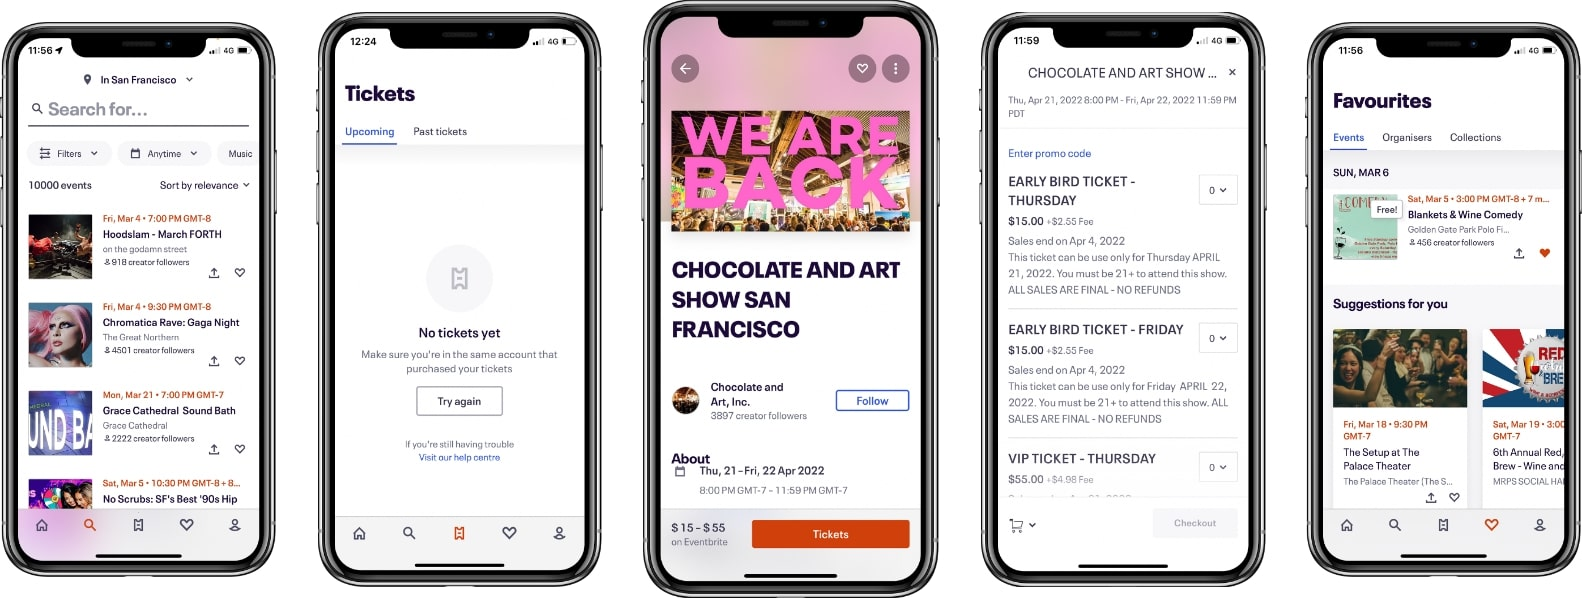
\includegraphics[scale=0.2]{slike/eventbrite.jpg} %veličina slike u odnosu na originalnu datoteku i pozicija slike
			\centering
			\caption{Sučelje aplikacije Eventbrite}
			\label{fig:eventBrite}
		\end{figure}


Za ovakvu aplikaciju mogle bi biti zainteresirane organizacije koje se bave promocijom događaja unutar neke domene. Npr. organizacije koje se bave organiziranjem tehno-partyja, javnih čitanja poezije ili bilo čega drugog. Time bi privukle publiku  koje baš takve određene teme zanimaju i osigurale da ih takva publika nađe lakše nego na već zakrčenom Facebooku. Velike firme ili fakulteti poput FER-a mogli bi ovu aplikaciju koristiti za oglašavanje događanja za svoje zaposlenike ili studente. Mjesta poput Velesajma ili Medike mogla bi koristiti ovakvu aplikaciju kao platformu koju bi organizatori događanja na takvim mjestima koristili za oglašavanje.

	U budućnosti bi se ovakva aplikacija mogla nadograditi na više načina.
 
	Moglo bi se omogućiti da se ne ocjenjuje samo događanja nego i njihove organizatore, tako da potencijalni posjetitelji mogu pretpostaviti koliko će kvalitetno događanje biti ne samo prema opisu i riječima organizatora, nego i po riječima onih koji su već imali iskustva s istim organizatorom.
 
	Također bi se mogla dodati funkcionalnost koja omogućuje oglašavanje poslova na oglašenim događanjima. Npr. ako na nekom događanju nedostaje konobar, organizator tog događanja moze tu informaciju dodati oglasu događanja. 
 
	Osim filtera koji postavljaju kriterije na mjesto i vrstu događaja, mogli bi se dodati filteri koji se odnose na organizatore događaja, njegov datum, dan u tjednu ili vrijeme u danu. Jedan od parametara filtera (i samih događaja)mogao bi biti i jezik na kojem će se događaj održati.

			
		
		%\textbf{\textit{dio 1. revizije}}\\
		
		\begin{comment}		
		\textit{Na osnovi projektnog zadatka detaljno opisati korisničke zahtjeve. Što jasnije opisati cilj projektnog zadatka, razraditi problematiku zadatka, dodati nove aspekte problema i potencijalnih rješenja. Očekuje se minimalno 3, a poželjno 4-5 stranica opisa.	Teme koje treba dodatno razraditi u ovom poglavlju su:}
		\begin{packed_item}
			\item \textit{potencijalna korist ovog projekta}
			\item \textit{postojeća slična rješenja (istražiti i ukratko opisati razlike u odnosu na zadani zadatak). Dodajte slike koja predočavaju slična rješenja.}
			\item \textit{skup korisnika koji bi mogao biti zainteresiran za ostvareno rješenje.}
			\item \textit{mogućnost prilagodbe rješenja }
			\item \textit{opseg projektnog zadatka}
			\item \textit{moguće nadogradnje projektnog zadatka}
		\end{packed_item}
		
		\textit{Za pomoć pogledati reference navedene u poglavlju „Popis literature“, a po potrebi konzultirati sadržaj na internetu koji nudi dobre smjernice u tom pogledu.}
		\eject)
		
		\section{Primjeri u \LaTeX u}
		
		\textit{Ovo potpoglavlje izbrisati.}\\

		U nastavku se nalaze različiti primjeri kako koristiti osnovne funkcionalnosti \LaTeX a koje su potrebne za izradu dokumentacije. Za dodatnu pomoć obratiti se asistentu na projektu ili potražiti upute na sljedećim web sjedištima:
		\begin{itemize}
			\item Upute za izradu diplomskog rada u \LaTeX u - \url{https://www.fer.unizg.hr/_download/repository/LaTeX-upute.pdf}
			\item \LaTeX\ projekt - \url{https://www.latex-project.org/help/}
			\item StackExchange za Tex - \url{https://tex.stackexchange.com/}\\
		
		\end{itemize} 	


		
		\noindent \underbar{podcrtani tekst}, \textbf{podebljani tekst}, 	\textit{nagnuti tekst}\\
		\noindent \normalsize primjer \large primjer \Large primjer \LARGE {primjer} \huge {primjer} \Huge primjer \normalsize
				
		\begin{packed_item}
			
			\item  primjer
			\item  primjer
			\item  primjer
			\item[] \begin{packed_enum}
				\item primjer
				\item[] \begin{packed_enum}
					\item[1.a] primjer
					\item[b] primjer
				\end{packed_enum}
				\item primjer
			\end{packed_enum}
			
		\end{packed_item}
		
		\noindent primjer url-a: \url{https://www.fer.unizg.hr/predmet/proinz/projekt}
		
		\noindent posebni znakovi: \# \$ \% \& \{ \} \_ 
		$|$ $<$ $>$ 
		\^{} 
		\~{} 
		$\backslash$ 
		
		
		\begin{longtblr}[
			label=none,
			entry=none
			]{
				width = \textwidth,
				colspec={|X[8,l]|X[8, l]|X[16, l]|}, 
				rowhead = 1,
			} %definicija širine tablice, širine stupaca, poravnanje i broja redaka naslova tablice
			\hline \SetCell[c=3]{c}{\textbf{naslov unutar tablice}}	 \\ \hline[3pt]
			\SetCell{LightGreen}IDKorisnik & INT	&  	Lorem ipsum dolor sit amet, consectetur adipiscing elit, sed do eiusmod  	\\ \hline
			korisnickoIme	& VARCHAR &   	\\ \hline 
			email & VARCHAR &   \\ \hline 
			ime & VARCHAR	&  		\\ \hline 
			\SetCell{LightBlue} primjer	& VARCHAR &   	\\ \hline 
		\end{longtblr}
		

		\begin{longtblr}[
				caption = {Naslov s referencom izvan tablice},
				entry = {Short Caption},
			]{
				width = \textwidth, 
				colspec = {|X[8,l]|X[8,l]|X[16,l]|}, 
				rowhead = 1,
			}
			\hline
			\SetCell{LightGreen}IDKorisnik & INT	&  	Lorem ipsum dolor sit amet, consectetur adipiscing elit, sed do eiusmod  	\\ \hline
			korisnickoIme	& VARCHAR &   	\\ \hline 
			email & VARCHAR &   \\ \hline 
			ime & VARCHAR	&  		\\ \hline 
			\SetCell{LightBlue} primjer	& VARCHAR &   	\\ \hline 
		\end{longtblr}
	


		
		
		%unos slike
		\begin{figure}[H]
			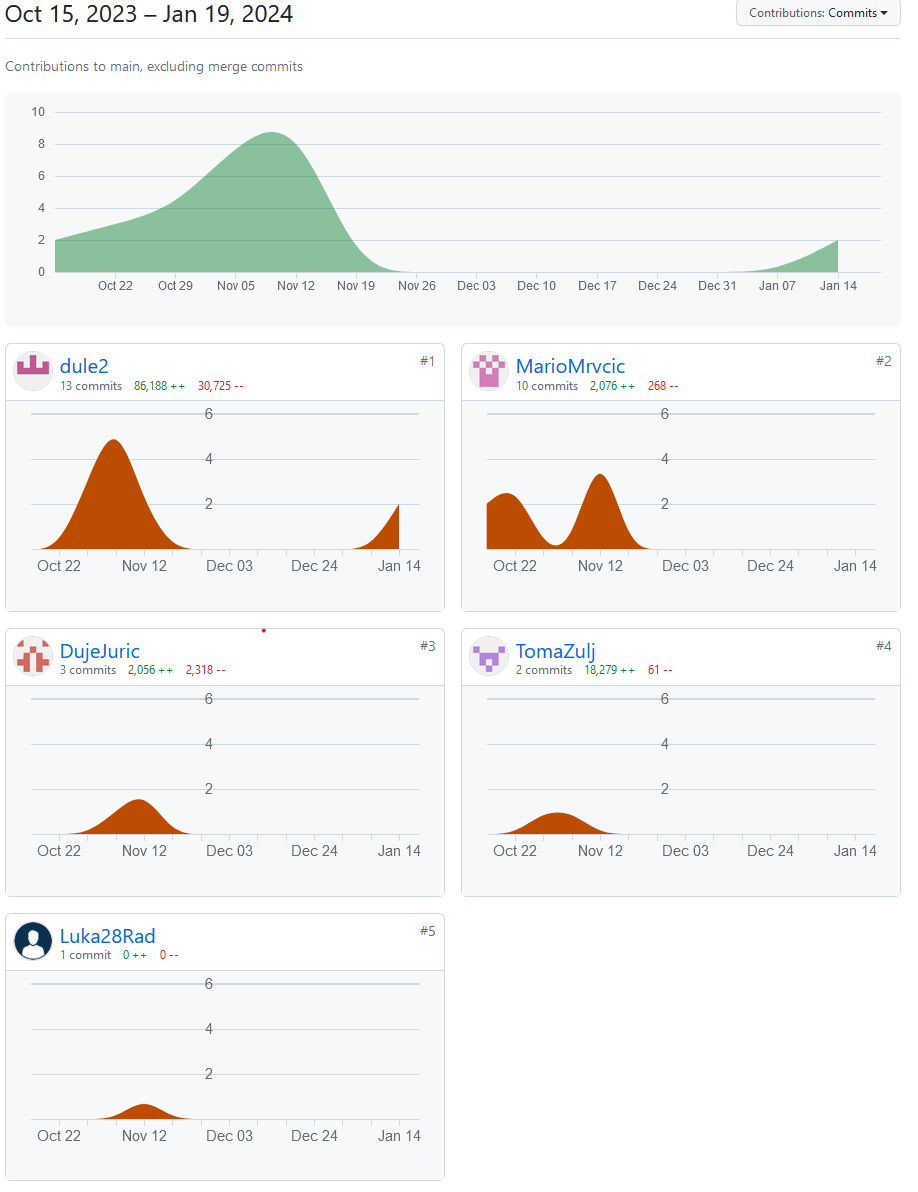
\includegraphics[scale=0.4]{slike/aktivnost.PNG} %veličina slike u odnosu na originalnu datoteku i pozicija slike
			\centering
			\caption{Primjer slike s potpisom}
			\label{fig:promjene}
		\end{figure}
		
		\begin{figure}[H]
			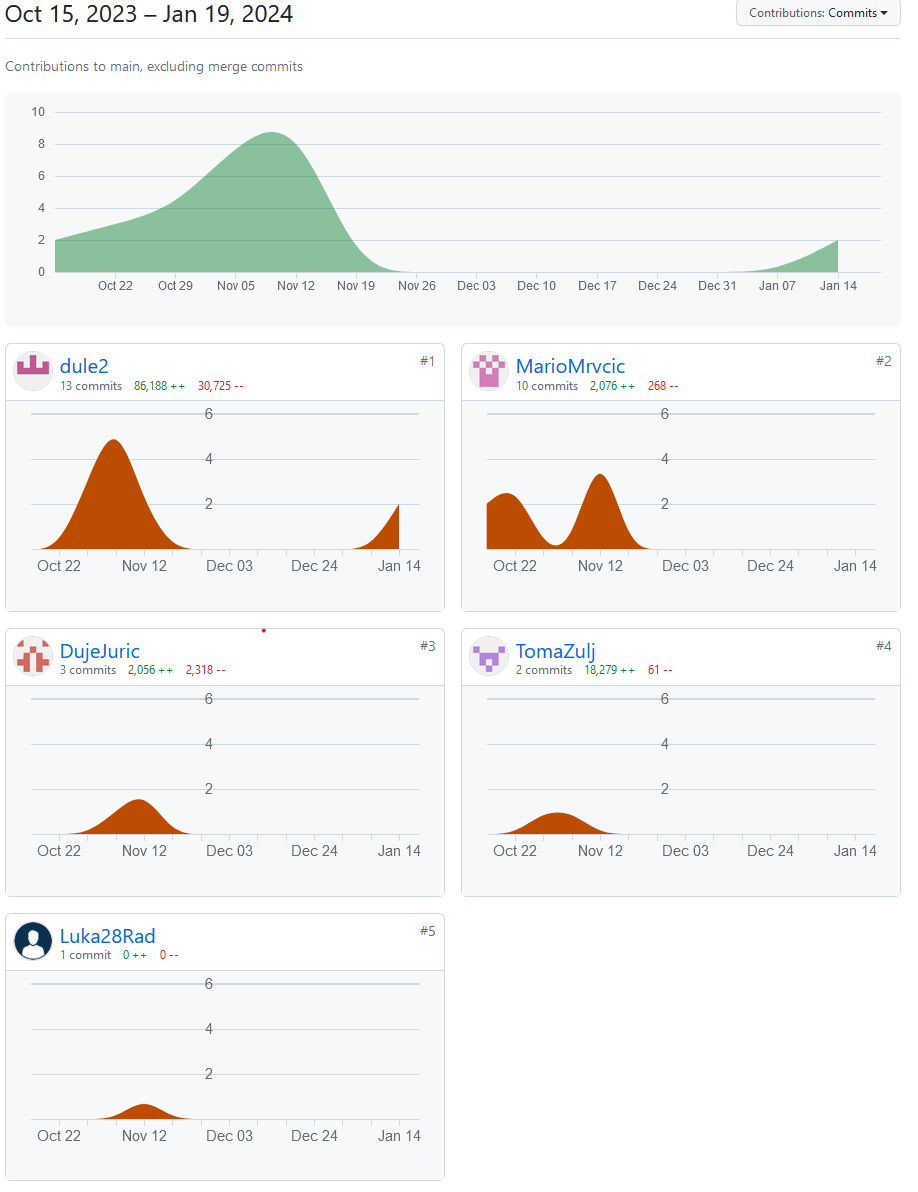
\includegraphics[width=\textwidth]{slike/aktivnost.PNG} %veličina u odnosu na širinu linije
			\caption{Primjer slike s potpisom 2}
			\label{fig:promjene2} %label mora biti drugaciji za svaku sliku
		\end{figure}
		
		Referenciranje slike \ref{fig:promjene2} u tekstu.
		
		\eject
		\end{comment}
	
	\chapter{Specifikacija programske potpore}
		
			
		
	\section{Funkcionalni zahtjevi}
			
			
			%\textbf{\textit{dio 1. revizije}}\\
			
			\textit{Navesti \textbf{dionike} koji imaju \textbf{interes u ovom sustavu} ili  \textbf{su nositelji odgovornosti}. To su prije svega korisnici, ali i administratori sustava, naručitelji, razvojni tim.}\\
				
			\textit{Navesti \textbf{aktore} koji izravno \textbf{koriste} ili \textbf{komuniciraju sa sustavom}. Oni mogu imati inicijatorsku ulogu, tj. započinju određene procese u sustavu ili samo sudioničku ulogu, tj. obavljaju određeni posao. Za svakog aktora navesti funkcionalne zahtjeve koji se na njega odnose.}\\
			
			
			\noindent \textbf{Dionici:}
			
			\begin{packed_enum}
				
				\item Posjetitelj
				\item Organizator			
				\item Administrator
				
			\end{packed_enum}
			
			\noindent \textbf{Aktori i njihovi funkcionalni zahtjevi:}
			
			
			\begin{packed_enum}
				\item  \underbar{Neregistrirani/neprijavljeni korisnik (inicijator) može:}
				
				\begin{packed_enum}
					
					\item pregled događanja
					\item odabir događanja i pregled općih informacija o događaju
					\item mogućnost registriranja kao posjetitelj, organizator ili administrator
					
				\end{packed_enum}
				
				\item  \underbar{Posjetitelj (inicijator) može:}
				
				\begin{packed_enum}
					
					\item pregled i mogućnost mijenjanja osobnih podataka
					\item brisanje vlastitog računa
					\item mogućnost ostavljanja recenzije na događaj
					\item mogućnost ostavljanja oznake zainteresiranosti za neki događaj
					\item mogućnost pretplaćivanja na obavjesti o budućim događanjima
					
					
				\end{packed_enum}
				
				\item  \underbar{Organizator (inicijator) može:}
				
				\begin{packed_enum}
									
					\item dodavanje događanja
					\item uređivanje informacija o svom događanju
					\item obaveza plaćanja članarine ako se događanja naplaćuju
					
					
				\end{packed_enum}
				
				\item  \underbar{Administrator (inicijator) može:}
				
				\begin{packed_enum}	
					
					\item  pregled svih registriranih korisnika i njihovih osobnih podataka
					\item  brisanje i mijenjanje uloga korisnika
					\item  pristup statistici događanja i korisnika
					\item  brisanje recenzija koje krše pravila korištenja
					\item  postavljanje cijene članarina organizatora
					
				\end{packed_enum}
			
				\item  \underbar{Baza podataka (sudionik) može:}
				
				\begin{packed_enum}
					
					\item pohranjuje sve podatke o korisnicima i njihovim ovlastima
					\item pohranjuje sve podatke o događajima
					
				\end{packed_enum}
				
				\item  \underbar{Banka (sudionik) može:}
				
				\begin{packed_enum}
					
					\item pruža mogućnost plaćanja članarine
					
				\end{packed_enum}
				
				\item  \underbar{Paypal (sudionik) može:}
				
				\begin{packed_enum}
					
					\item pruža mogućnost plaćanja članarine
					
				\end{packed_enum}
			\end{packed_enum}
			
			\eject 
			
			
				
			\subsection{Obrasci uporabe}
				
				\textbf{\textit{dio 1. revizije}}
				
				\subsubsection{Opis obrazaca uporabe}
					\textit{Funkcionalne zahtjeve razraditi u obliku obrazaca uporabe. Svaki obrazac je potrebno razraditi prema donjem predlošku. Ukoliko u nekom koraku može doći do odstupanja, potrebno je to odstupanje opisati i po mogućnosti ponuditi rješenje kojim bi se tijek obrasca vratio na osnovni tijek.}\\
					

					\noindent \underbar{\textbf{UC1 -Pregled događanja}}
					\begin{packed_item}
	
						\item \textbf{Glavni sudionik: }Korisnik, posjetitelj
						\item  \textbf{Cilj:} Pregled ponude događanja
						\item  \textbf{Sudionici:} Baza podataka
						\item  \textbf{Preduvjet:} -
						\item  \textbf{Opis osnovnog tijeka:}
						
						\item[] \begin{packed_enum}
	
							\item prikaz početnog zaslona sa popisom događanja
							\item korisnik bira događanje 
							\item prikaz informacija i galerije događanja
							\item mogućnost registracije i prijave
						\end{packed_enum}
						
					\end{packed_item}
					
					\noindent \underbar{\textbf{UC2 -Registracija}}
					\begin{packed_item}
	
						\item \textbf{Glavni sudionik: }Korisnik
						\item  \textbf{Cilj:} Stvaranje korisničkog računa
						\item  \textbf{Sudionici:} Baza podataka
						\item  \textbf{Preduvjet:} -
						\item  \textbf{Opis osnovnog tijeka:}
						
						\item[] \begin{packed_enum}
	
							\item odabir opcije za registraciju 
							\item unos osobnih podatak, postavljanje lozinke i odabir uloge
							\item dobivanje povratne informacije o uspješnoj registraciji
							
						\end{packed_enum}
						
						\item  \textbf{Opis mogućih odstupanja:}
						
						\item[] \begin{packed_item}
	
							\item[2.a] Unos već postojećeg emaila ili korisničkog imena, unos podatka u nezadovoljavajućem formatu
							\item[] \begin{packed_enum}
								
								\item obavjest o pogrešnom unosu
								\item ponovni unos potrebnih podataka
								
							\end{packed_enum}
							
							
						\end{packed_item}
					\end{packed_item}
					
					\noindent \underbar{\textbf{UC3 -Prijava u sustav}}
					\begin{packed_item}
	
						\item \textbf{Glavni sudionik: }Posjetitelj
						\item  \textbf{Cilj:} Prijava u vlastiti korisnički račun
						\item  \textbf{Sudionici:} Baza podataka
						\item  \textbf{Preduvjet:} obavljena registracija
						\item  \textbf{Opis osnovnog tijeka:}
						
						\item[] \begin{packed_enum}
	
							\item odabir opcije za prijavu 
							\item unos korisničkog imena i lozinke
							\item pristup funkcionalnostima korisničkog računa
							
						\end{packed_enum}
						
						\item  \textbf{Opis mogućih odstupanja:}
						
						\item[] \begin{packed_item}
	
							\item[2.a] neispravno korisničko ime ili lozinka
							\item[] \begin{packed_enum}
								
								\item obavijest o pogrešnom unosu korisničkog imena ili lozinke
								\item ponovni unos potrebnih podataka
								
							\end{packed_enum}
							
						\end{packed_item}
					\end{packed_item}
					
					\noindent \underbar{\textbf{UC4 -Pregled osobnih podataka}}
					\begin{packed_item}
	
						\item \textbf{Glavni sudionik: }Posjetitelj
						\item  \textbf{Cilj:} Uvid u vlastite osobne podatke
						\item  \textbf{Sudionici:} Baza podataka
						\item  \textbf{Preduvjet:} posjetitelj je prijavljen
						\item  \textbf{Opis osnovnog tijeka:}
						
						\item[] \begin{packed_enum}
	
							\item odabir opcije pregleda osobnih podataka
							\item uvid u osobne podatke
							
						\end{packed_enum}
					\end{packed_item}
					
					\noindent \underbar{\textbf{UC5 -Promjena osobnih podataka}}
					\begin{packed_item}
	
						\item \textbf{Glavni sudionik: }Posjetitelj
						\item  \textbf{Cilj:} izmjena vlastitih osobnih podataka
						\item  \textbf{Sudionici:} Baza podataka
						\item  \textbf{Preduvjet:} posjetitelj je prijavljen
						\item  \textbf{Opis osnovnog tijeka:}
						
						\item[] \begin{packed_enum}
	
							\item odabir opcije za izmjenu podataka
							\item izmjena podataka
							\item spremanje podataka 
							\item ažuriranje baze
							
						\end{packed_enum}
						
						\item  \textbf{Opis mogućih odstupanja:}
						
						\item[] \begin{packed_item}
	
							\item[2.a] opcije za spremanje podataka nije odabrana
							\item[] \begin{packed_enum}
								
								\item obavijest o opasnosti da se podatci neće spremiti
								
							\end{packed_enum}
						
							
						\end{packed_item}
					\end{packed_item}
					
					\noindent \underbar{\textbf{UC6 -Brisanje korisničkog računa}}
					\begin{packed_item}
	
						\item \textbf{Glavni sudionik: }Posjetitelj 
						\item  \textbf{Cilj:} brisanje vlastitog korisničkog računa
						\item  \textbf{Sudionici:} Baza podataka
						\item  \textbf{Preduvjet:} posjetitelj je prijavljen
						\item  \textbf{Opis osnovnog tijeka:}
						
						\item[] \begin{packed_enum}
	
							\item odabir opcije za uređivanuje računa
							\item odabir opcije za brisanje računa
							\item korisnički račun se briše iz baze
							\item otvara se početna stranica 
							
						\end{packed_enum}

					\end{packed_item}
					
					\noindent \underbar{\textbf{UC7 -Reakcija na događanje}}
					\begin{packed_item}
	
						\item \textbf{Glavni sudionik: }Posjetitelj 
						\item  \textbf{Cilj:} naznaka o dolaznosti posjetitelja
						\item  \textbf{Sudionici:} Baza podataka
						\item  \textbf{Preduvjet:} posjetitelj je prijavljen
						\item  \textbf{Opis osnovnog tijeka:}
						
						\item[] \begin{packed_enum}
	
							\item odabir opcije za reakciju na određenom događaju 
							\item mogućnost odabira jedne od opcija: "Dolazim", "Ne dolazim" i "Možda dolazim"
						\end{packed_enum}

					\end{packed_item}
					
					\noindent \underbar{\textbf{UC8 -Dodavanje recenzije}}
					\begin{packed_item}
	
						\item \textbf{Glavni sudionik: }Posjetitelj 
						\item  \textbf{Cilj:} dodavanje recenzije na događaj
						\item  \textbf{Sudionici:} Baza podataka
						\item  \textbf{Preduvjet:} 
						\item[] \begin{packed_enum}
								
								\item posjetitelj je prijavljen
								\item opcija je odabrana u manje od 48 sati od završetka događanja
								\item posjetitelj je predhodno označio događaj s: "Dolazim" ili "Možda dolazim" 
								
							\end{packed_enum}
							
						\item  \textbf{Opis osnovnog tijeka:}
						
						\item[] \begin{packed_enum}
	
							\item odabir opcije za dodavanje recenzije 
							\item pisanje recenzije
							\item spremanje recenzije na bazu podataka
							
						\end{packed_enum}
						
					\end{packed_item}
					
					\noindent \underbar{\textbf{UC9 -Pregled recenzija}}
					\begin{packed_item}
	
						\item \textbf{Glavni sudionik: }Posjetitelj
						\item  \textbf{Cilj:} Uvid u ocjene prijašnjih događanja
						\item  \textbf{Sudionici:} Baza podataka
						\item  \textbf{Preduvjet:} -
						\item  \textbf{Opis osnovnog tijeka:}
						
						\item[] \begin{packed_enum}
	
							\item odabir opcije za prikaz recenzija određenog događaja
							\item prikaz svih recenzija poredanih od najnovije
							
						\end{packed_enum}
					\end{packed_item}
					
					
					
					\noindent \underbar{\textbf{UC10 -Prijava na obavjesti}}
					\begin{packed_item}
	
						\item \textbf{Glavni sudionik: }Posjetitelj
						\item  \textbf{Cilj:} prijava posjetitelja na primanje obavjesti o budućim događanjima
						\item  \textbf{Sudionici:} Baza podataka
						\item  \textbf{Preduvjet:} posjetitelj je prijavljen
						\item  \textbf{Opis osnovnog tijeka:}
						
						\item[] \begin{packed_enum}
	
							\item odabir opcije za prijavljivanje na obavjesti
							\item odabir parametara prema kojima posjetitelj želi primati obavjesti
						\end{packed_enum}
						
					\end{packed_item}
					
					\noindent \underbar{\textbf{UC11 -Uređivanje događanja korisnika}}
					\begin{packed_item}
	
						\item \textbf{Glavni sudionik: }Posjetitelj
						\item  \textbf{Cilj:} uređivanje odabira na događanjima za koje je posjetitelj zainteresiran
						\item  \textbf{Sudionici:} Baza podataka
						\item  \textbf{Preduvjet:} posjetitelj je prijavljen
						\item  \textbf{Opis osnovnog tijeka:}
						
						\item[] \begin{packed_enum}
	
							\item odabir opcije za uređivanje vlastitih događanja
							\item odabir događanja za koje se žele izvršiti promjene
							\item izmjena zainteresiranosti ili recenzije za određeno događanje 
							
						\end{packed_enum}
						
					\end{packed_item}
					
					\noindent \underbar{\textbf{UC12 -Obavjest o nadolazećem događanju}}
					\begin{packed_item}
	
						\item \textbf{Glavni sudionik: }Baza podataka 
						\item  \textbf{Cilj:} Poslati obavjest posjetitelju 
						\item  \textbf{Sudionici:} Posjetitelj
						\item  \textbf{Preduvjet:} Posjetitelj mora zadovoljavati uvjete koji su zadani događajem
						\item  \textbf{Opis osnovnog tijeka:}
						
						\item[] \begin{packed_enum}
	
							\item podatci o novonastalom događaju zadovoljavaju ujete koje su određeni posjetitelji označili kao poželjne
							\item baza podataka šalje informacije o događaju svim zainteresiranim posjetiteljima
							\item posjetiteljima na uređaju dolazi obavjest o događanju
						\end{packed_enum}
						
					\end{packed_item}
					
					\noindent \underbar{\textbf{UC13 -Kreacija događanja}}
					\begin{packed_item}
	
						\item \textbf{Glavni sudionik: }Organizator 
						\item  \textbf{Cilj:} stvaranje novog događanja
						\item  \textbf{Sudionici:} Baza podataka
						\item  \textbf{Preduvjet:} organizator je prijavljen
						\item  \textbf{Opis osnovnog tijeka:}
						
						\item[] \begin{packed_enum}
	
							\item odabir opcije za kreiranje novog događanja
							\item unos podataka, fotografija i cijeni ulaznica za buduće događanje
							\item spremanje podataka
						\end{packed_enum}
						
						\item  \textbf{Opis mogućih odstupanja:}
						
						\item[] \begin{packed_item}
	
							\item[2.a] ulaznice se plaćaju
							\item[] \begin{packed_enum}
								
								\item ako organizator nije uplatio članarinu otvara mu se stranica za uplatu
								\item organizator potvrđuje da želi naplaćivati ulaznice i sprema svoj odabir
								
							\end{packed_enum}
							
							
						\end{packed_item}
					\end{packed_item}
					
					\noindent \underbar{\textbf{UC14 -Uređivanje događanja}}
					\begin{packed_item}
	
						\item \textbf{Glavni sudionik: }Organizator
						\item  \textbf{Cilj:} Uzmjena podataka o vlastitom događaju
						\item  \textbf{Sudionici:} Baza podataka
						\item  \textbf{Preduvjet:} Organizator je prijavljen i događanje još nije završilo
						\item  \textbf{Opis osnovnog tijeka:}
						
						\item[] \begin{packed_enum}
	
							\item odabir događanja na kojem se žele napraviti izmjene
							\item izmjena podataka
							\item spremanje izmjena na bazu podataka
							
						\end{packed_enum}
						
						\item  \textbf{Opis mogućih odstupanja:}
						
						\item[] \begin{packed_item}
	
							\item[2.a] događanje je s besplatnog dobilo cjenu ulaznice
							\item[] \begin{packed_enum}
								
								\item provjerava se jeli članarina uplačena
								\item ako članarina nije uplačena korisnik se odvodi na stranicu za uplatu članarine
								
							\end{packed_enum}
						\end{packed_item}
							
					\end{packed_item}
					
					\noindent \underbar{\textbf{UC15 -Odgovaranje na recenzije}}
					\begin{packed_item}
	
						\item \textbf{Glavni sudionik: }Organizator
						\item  \textbf{Cilj:} odgovaranje na recenzije koje su posjtitelji ostavili na njegovo događanje
						\item  \textbf{Sudionici:} Baza podataka
						\item  \textbf{Preduvjet:} organizator je prijavljen
						\item  \textbf{Opis osnovnog tijeka:}
						
						\item[] \begin{packed_enum}
	
							\item odabir popisa recenzija na vlastitom događanju 
							\item odabir recenzije na koju želi dati odgovor
							\item pisanje odgovora na recenziju 
							\item spremanje u bazu podataka
							
						\end{packed_enum}

					\end{packed_item}
					
					\noindent \underbar{\textbf{UC16 -Plaćanje članarine}}
					\begin{packed_item}
	
						\item \textbf{Glavni sudionik: }Organizator
						\item  \textbf{Cilj:} Plaćanje članarine organizatora
						\item  \textbf{Sudionici:} Baza podataka, Paypal, Banka
						\item  \textbf{Preduvjet:} organizator ima barem 1 događaj za koji se naplačuju karte
						\item  \textbf{Opis osnovnog tijeka:}
						
						\item[] \begin{packed_enum}
	
							\item odabir opcije za uplatu članarine
							\item odabir načina plačanja 
							\item plačanje članarine
							\item potvrda o uspješnoj uplati članarine
						\end{packed_enum}
						
						\item  \textbf{Opis mogućih odstupanja:}
						
						\item[] \begin{packed_item}
	
							\item[2.a] neuspješna uplata
							\item[] \begin{packed_enum}
								
								\item obavjest o neuspješnoj transakciji
								\item opcije za ponovni pokušaj ili za odustajanje od uplate
								
							\end{packed_enum}
							
					\end{packed_item}
					
					
					\noindent \underbar{\textbf{UC17 -Brisanje događanja}}
					\begin{packed_item}
	
						\item \textbf{Glavni sudionik: }Organizator
						\item  \textbf{Cilj:} Brisanje vlastitog događanja
						\item  \textbf{Sudionici:} Baza podataka
						\item  \textbf{Preduvjet:}Organizator je prijavljen
						\item  \textbf{Opis osnovnog tijeka:}
						
						\item[] \begin{packed_enum}
	
							\item odabir događanja na kojem se žele napraviti izmjene
							\item odabire opciju za brisanje događanja
							\item povratak na glavnu stranicu
							
						\end{packed_enum}
						
					\end{packed_item}
					
					
					
					\noindent \underbar{\textbf{UC18 -Pregled korisnika}}
					\begin{packed_item}
	
						\item \textbf{Glavni sudionik: }Administrator 
						\item  \textbf{Cilj:} uvid u podatke o korisnicima
						\item  \textbf{Sudionici:} Baza podataka
						\item  \textbf{Preduvjet:} administrator je prijavljen
						\item  \textbf{Opis osnovnog tijeka:}
						
						\item[] \begin{packed_enum}
	
							\item odabir opcije za pregled korisnika
							\item prikaz popisa korisnika i njohovih podataka
						\end{packed_enum}
						
						
					\end{packed_item}
					
					\noindent \underbar{\textbf{UC19 -Brisanje korisnika}}
					\begin{packed_item}
	
						\item \textbf{Glavni sudionik: }Administrator, 
						\item  \textbf{Cilj:} Brisanje određenog korisničkog računa
						\item  \textbf{Sudionici:} Baza podataka
						\item  \textbf{Preduvjet:} administrator je prijavljen
						\item  \textbf{Opis osnovnog tijeka:}
						
						\item[] \begin{packed_enum}
	
							\item odabir opcije za pregled korisnika
							\item odabir korisnika koji se treba obrisati
							\item odabir opcije za brisanje korisnika
						\end{packed_enum}
						
					\end{packed_item}
					
					\noindent \underbar{\textbf{UC20 -Postavljanje cijene članarine}}
					\begin{packed_item}
	
						\item \textbf{Glavni sudionik: }Administrator
						\item  \textbf{Cilj:} Postavljanje cijene članarine koju plaćaju organizatori
						\item  \textbf{Sudionici:} Baza podataka
						\item  \textbf{Preduvjet:} administrator je prijavljen
						\item  \textbf{Opis osnovnog tijeka:}
						
						\item[] \begin{packed_enum}
	
							\item odabir opcije za izmjenu cije članarine 
							\item izmjena cijene članarine
						\end{packed_enum}
						
						
					\end{packed_item}
					
					\noindent \underbar{\textbf{UC21 -Uređivanje određenog događanja}}
					\begin{packed_item}
	
						\item \textbf{Glavni sudionik: }Administrator
						\item  \textbf{Cilj:} uređivanje određenog događanja
						\item  \textbf{Sudionici:} Baza podataka
						\item  \textbf{Preduvjet:} administrator je prijavljen
						\item  \textbf{Opis osnovnog tijeka:}
						
						\item[] \begin{packed_enum}
	
							\item iz prikaza svih događanja odabire se željeni događaj
							\item odabire se opcija uređivanja događanja
							\item spremaju se promjene
							\item povratak na prikaz svih događanja
						\end{packed_enum}
						\item  \textbf{Opis mogućih odstupanja:}
						
						\item[] \begin{packed_item}
	
							\item[3.a] administrator želi promjeniti cijenu ulaznice s 0 na broj veći od 0
							\item[] \begin{packed_enum}
								
								\item promjena nije moguća
								
							\end{packed_enum}
						
							
						\end{packed_item}
							
					\end{packed_item}
					
					\noindent \underbar{\textbf{UC22 -Brisanje određenog događanja}}
					\begin{packed_item}
	
						\item \textbf{Glavni sudionik: }Administrator
						\item  \textbf{Cilj:} brisanje određenog događanja
						\item  \textbf{Sudionici:} Baza podataka
						\item  \textbf{Preduvjet:} administrator je prijavljen
						\item  \textbf{Opis osnovnog tijeka:}
						
						\item[] \begin{packed_enum}
	
							\item iz prikaza svih događanja odabire se željeni događaj
							\item odabire se opcija brisanja događanja
							\item povratak na prikaz svih događanja
						\end{packed_enum}
							
					\end{packed_item}
					
					
					
					\noindent \underbar{\textbf{UC23 -Brisanje recenzija}}
					\begin{packed_item}
	
						\item \textbf{Glavni sudionik: }Administrator
						\item  \textbf{Cilj:} Brisanje recenzija koje ne poštuju preavila korištenja
						\item  \textbf{Sudionici:} Baza podataka
						\item  \textbf{Preduvjet:} administrator je prijavljen
						\item  \textbf{Opis osnovnog tijeka:}
						
						\item[] \begin{packed_enum}
	
							\item odabir opcije za prikaz recenzija određenog događanja
							\item odabir recenzije
							\item odabir opcije za brisanje recenzije
						\end{packed_enum}
						
						\end{packed_item}
					\end{packed_item}
					
					
					\noindent \underbar{\textbf{UC24 -Promjena uloge}}
					\begin{packed_item}
	
						\item \textbf{Glavni sudionik: }Administrator
						\item  \textbf{Cilj:} Izmjena uloge određenog korisnika
						\item  \textbf{Sudionici:} Baza podataka
						\item  \textbf{Preduvjet:} administrator je prijavljen 
						\item  \textbf{Opis osnovnog tijeka:}
						
						\item[] \begin{packed_enum}
	
							\item odabir popisa svih korisnika
							\item odabir korisnika kojemu se želi pormjeniti uloga
							\item odabir opcije za izmjenu uloge
							\item odabir uloge koja mu se dodjeljuje
						\end{packed_enum}
						
					\end{packed_item}
					\noindent \underbar{\textbf{UC23 -Pregled statistike}}
					\begin{packed_item}
	
						\item \textbf{Glavni sudionik: }Administrator
						\item  \textbf{Cilj:} Uvid u statistiku svih aktera u aplikaciji
						\item  \textbf{Sudionici:} Baza podataka
						\item  \textbf{Preduvjet:} administrator je pirjavljen
						\item  \textbf{Opis osnovnog tijeka:}
						
						\item[] \begin{packed_enum}
	
							\item odabir opcije za prikaz statistike
							\item prikaz statistike
						\end{packed_enum}
						
					\end{packed_item}
					
					
					
					
					
					
				
					
				\subsubsection{Dijagrami obrazaca uporabe}
					
					\textit{Prikazati odnos aktora i obrazaca uporabe odgovarajućim UML dijagramom. Nije nužno nacrtati sve na jednom dijagramu. Modelirati po razinama apstrakcije i skupovima srodnih funkcionalnosti.}
				\eject		
				
			\subsection{Sekvencijski dijagrami}
				
				\textbf{\textit{dio 1. revizije}}\\
				
				\textit{Nacrtati sekvencijske dijagrame koji modeliraju najvažnije dijelove sustava (max. 4 dijagrama). Ukoliko postoji nedoumica oko odabira, razjasniti s asistentom. Uz svaki dijagram napisati detaljni opis dijagrama.}
				\eject
	
		\section{Ostali zahtjevi}
		
			\textbf{\textit{dio 1. revizije}}\\
		 
			 \textit{Nefunkcionalni zahtjevi i zahtjevi domene primjene dopunjuju funkcionalne zahtjeve. Oni opisuju \textbf{kako se sustav treba ponašati} i koja \textbf{ograničenja} treba poštivati (performanse, korisničko iskustvo, pouzdanost, standardi kvalitete, sigurnost...). Primjeri takvih zahtjeva u Vašem projektu mogu biti: podržani jezici korisničkog sučelja, vrijeme odziva, najveći mogući podržani broj korisnika, podržane web/mobilne platforme, razina zaštite (protokoli komunikacije, kriptiranje...)... Svaki takav zahtjev potrebno je navesti u jednoj ili dvije rečenice.}
			 
			 
			 
	
	\chapter{Arhitektura i dizajn sustava}
		\begin{comment}
		\textbf{\textit{dio 1. revizije}}\\

		\textit{ Potrebno je opisati stil arhitekture te identificirati: podsustave, preslikavanje na radnu platformu, spremišta podataka, mrežne protokole, globalni upravljački tok i sklopovsko-programske zahtjeve. Po točkama razraditi i popratiti odgovarajućim skicama:}
	\begin{itemize}
		\item 	\textit{izbor arhitekture temeljem principa oblikovanja pokazanih na predavanjima (objasniti zašto ste baš odabrali takvu arhitekturu)}
		\item 	\textit{organizaciju sustava s najviše razine apstrakcije (npr. klijent-poslužitelj, baza podataka, datotečni sustav, grafičko sučelje)}
		\item 	\textit{organizaciju aplikacije (npr. slojevi frontend i backend, MVC arhitektura) }		
	\end{itemize}
	\end{comment}
	
	Arhitekturu sustava našeg projekta možemo podijeliti na tri glavna podsustava:
	
	\begin{packed_enum}
	
		\item Baza podataka
		\item Web aplikacija
		\item Web poslužitelj
		
	
	\begin{figure}[H]
			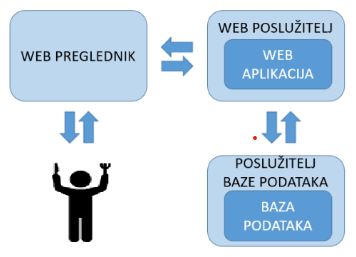
\includegraphics[scale=0.8]{slike/Arhitektura.png} %veličina slike u odnosu na originalnu datoteku i pozicija slike
			\centering
			\caption{Skica arhitekture sustava}
			\label{fig:ARH}
		\end{figure}
		
		
							
	\end{packed_enum}
	
	Internetski preglednik predstavlja programsku platformu koja korisnicima omogućuje pregledavanje web-stranica i konzumiranje raznovrsnih multimedijalnih sadržaja povezanih s njima. Svaki od tih preglednika funkcionira kao svojevrsni tumač, čime interpretira kompleksni kod web stranica i pretvara ga u vizualno prihvatljiv format za korisnike. Bitno je razumjeti da je ključna uloga internetskog preglednika prevesti tehnički zahtjevne  elemente weba u nešto pristupačno svakom korisniku.
	
	Kada korisnik putem internetskog preglednika šalje zahtjev, ta komunikacija se uspostavlja s web poslužiteljem. Web poslužitelj predstavlja temelj rada web aplikacija, a njegova osnovna zadaća je posredovati u komunikaciji između korisnika (klijenta) i same aplikacije. Cijeli taj proces komunikacije odvija se putem HTTP (HyperText Transfer Protocol) protokola, koji služi kao standardni način prijenosa informacija na internetu.

	Važno je naglasiti da je web poslužitelj taj koji pokreće web aplikaciju i prosljeđuje joj korisnički zahtjev. Kroz korištenje web aplikacije, korisnik šalje različite zahtjeve koje aplikacija obrađuje. Ovisno o konkretnom zahtjevu, web aplikacija može pristupiti bazi podataka kako bi došla do relevantnih informacija. Nakon obrade zahtjeva, aplikacija putem web poslužitelja šalje odgovor korisniku u obliku HTML dokumenta. Taj dokument postaje vizualno doživljajan u internetskom pregledniku, predstavljajući krajnji rezultat korisničkog zahtjeva.
	
	Programski jezik kojeg smo odabrali za izradu naše web aplikacije je Java zajedno s React i Spring Boot stackom. Projekt programiramo u razvojnom okruženju Intellj IDEA. Arhitekturu sustava baziramo na MVC konceptu (Model-View-Controller) prilagođenom za React i Spring boot. Glavna karakteristika zbog koje smo se odlučili za MVC je nezavisno razvijanje pojedinih dijelova aplikacije što nam omogućuje jednostavnije testiranje i implementiranje novog koda. Glavna podjela je na tzv. „Backend“ i „Frontend“.
	\vspace{30pt}
	
	
	Backend (Spring Boot) MVC koncept:
	
	\begin{packed_enum}
	
		\item Model: Svi razredi (koje su povezane sa bazom) sa odgovarajućim atributima te servisi u kojima se provodi logika koji kasnije koriste API komponente (Controlleri)
		\item View: JSON podatci s kojima upravljaju API komponente(Controlleri)
		\item Controller: API komponente koje obrađuju zahtjeve te šalju adekvatne odgovore
							
	\end{packed_enum}
	\eject
	
	Frontend (React) MVC arhitektura:
	
	\begin{packed_enum}
	
		\item Model: Stanja i podatci koje se koriste i prikazuju u komponentama
		\item View: Komponente koje reprezentiraju izgled aplikacije odnosno korisničko sučelje
		\item Controller: „Event handleri“ i metode koje obrađuju logiku, unos korisnika te upravljaju podatcima i stanjima u komponentama 
							
	\end{packed_enum}
		

				
		\section{Baza podataka}
			
			Za potrebe našeg sustava koristit ćemo bazu podataka koja svojom strukturom olakšava modeliranje stvarnog svijeta. Osnovna jedinica baze je dokument, definiran svojim imenom i skupom atributa. Dokument može nadovezivati i klasa koja opisuje atribute sadržane u dokumentu. Korištenjem MongoDB-a kao ne-relacijske baze podataka, informacije će biti pohranjene u obliku fleksibilnih dokumenata umjesto tradicionalnih tablica. Zadaća baze podataka je brza i jednostavna pohrana, izmjena i dohvat podataka za daljnju obradu. Baza podataka ove aplikacije sastoji se od sljedećih dokumenata te klasa koje su sadržane unutar njih:
			\begin{packed_item}
	
						\item Korisnik
						
						\item Događanje
							\begin{packed_item}
							\item Mjesto
							\item Foto (lista)
							\item Video (lista)
							\item Recenzije (lista)
							\end{packed_item}
						
						\item Korisnik-Događanje
						
						
						
			\end{packed_item}
			
			Osim dokumenata i klasa u bazi ćemo također imati i vlastite tipove podataka koje će biti prethodno definirani. To su: 
			\begin{packed_item}
	
						\item Uloga
						\item Vrsta
						\item Interes
			\end{packed_item}
						
				
			\subsection{Opis tablica}
			
			\textbf{\large Dokumenti}\\
			

			
			
				%\textit{Svaku tablicu je potrebno opisati po zadanom predlošku. Lijevo se nalazi točno ime varijable u bazi podataka, u sredini se nalazi tip podataka, a desno se nalazi opis varijable. Svjetlozelenom bojom označite primarni ključ. Svjetlo plavom označite strani ključ}
				\textbf{Korisnik} Ovaj dokument sadrži informacije o pojedinačnom korisniku. Sadrži atribute: email, lozinku, ime, prezime, adresu, ulogu, gradove interesa, vrste interesa, web stranicu i facebook. Ovaj dokument je u vezi \textit{One-to-Many} s dokumentom Korisnik-Događanje preko atributa email. Pošto je baza nerelacijska u dokument će se također pisati i liste od: gradova i vrsta koje su potrebne kako bi se izvele sve funkcionalnosti.  
				
				
				
				\begin{longtblr}[
					label=none,
					entry=none
					]{
						width = \textwidth,
						colspec={|X[6,l]|X[10, l]|X[20, l]|}, 
						rowhead = 1,
					} %definicija širine tablice, širine stupaca, poravnanje i broja redaka naslova tablice
					\hline \SetCell[c=3]{c}{\textbf{Korisnik}}	 \\ \hline[3pt]
					\SetCell{LightGreen}Email & STRING	& email korisnika \\ \hline 
					Lozinka	& STRING & hash lozinke\\ \hline 
					Ime	& STRING &   ime korisnika	\\ \hline 
					Prezime & STRING &  prezime korisnika \\ \hline
					Adresa & STRING & kućna adresa korisnika \\ \hline 
					Uloga & ULOGA & uloga korisnika	\\ \hline 
					Gradovi interesa & LIST$<$STRING$>$ & gradovi interesa korisnika \\ \hline 
					Vrste interesa & LIST$<$VRSTA$>$ & vrste interesa korisnika \\ \hline  
					Web stranica & STRING & link web stranice organizatora \\ \hline 
					Facebook & STRING & link facebook profila organizatora \\ \hline
					\end{longtblr}
				
		
			

				\textbf{Događanje} Ovaj dokument sadrži informacije o pojedinačnom događanju. Sadrži atribute: ID, ime, vrsta, mjesto, adresu, datum, vrijeme početka, trajanje, opis, cijenu, foto galeriju, video galeriju i recenzije. Ovaj je dokument u vezi \textit{One-to-Many} s dokumentom Korisnik-Događanje preko atribute ID. Događanje se također nadovezuje na klase mjesto, foto, video i recenziju. Za mjesto bi se moglo reći da je u vezi \textit{One-to-One} jer ima samo jedno mjesto na kojem se događaj može odvijati, a za foto, video i recenzije bi se moglo reći da je u vezi \textit{One-to-Many} jer može imati po više takvih atributa. Zato su ti atributi zapisani u listi.
				
				
				\begin{longtblr}[
					label=none,
					entry=none
					]{
						width = \textwidth,
						colspec={|X[6,l]|X[12, l]|X[20, l]|}, 
						rowhead = 1,
					} %definicija širine tablice, širine stupaca, poravnanje i broja redaka naslova tablice
					\hline \SetCell[c=3]{c}{\textbf{Događanje}}	 \\ \hline[3pt]
					\SetCell{LightGreen}ID & LONG &  	jedinstveni identifikator događanja\\ \hline
					Ime	& STRING &   ime događanja	\\ \hline 
					Vrsta & VRSTA &  vrsta događanja \\ \hline 
					Mjesto & MJESTO	&  grad događanja	\\ \hline 
					Adresa & STRING	& adresa događanja \\ \hline 
					Datum & DATE & datum održavanja	\\ \hline 
					Vrijeme početka & LOCALTIME & vrijeme početka održavanja \\ \hline 
					Trajanje & LOCALTIME & trajanje događanja \\ \hline 
					Opis & STRING & opis događanja \\ \hline 
					Cijena & DOUBLE	&  cijena ulaznice	\\ \hline 
					\SetCell{LightPink}Foto galerija & LIST$<$FOTO$>$ & fotografije događanja \\ \hline 
					\SetCell{LightPink}Video galerija & LIST$<$VIDEO$>$ & videozapisi događanja \\ \hline
					\SetCell{LightPink}Recenzije & LIST$<$RECENZIJA$>$ & recenzije događanja \\ \hline
					\end{longtblr}
				

				\textbf{Korisnik-Događanje}	Ovaj dokument sadrži informacije o odnosu korisnika i događanja. Glavna zadaća mu je da čuva informaciju o tome koji se korisnik izjasni da će doći na koje događanje. Sadrži atribute: email, ID i interes. Sa korisnikom i sa događanjem je povezan \textit{Many-to-One} vezom preko emaila i IDa.
				
				
				\begin{longtblr}[
					label=none,
					entry=none
					]{
						width = \textwidth,
						colspec={|X[6,l]|X[6, l]|X[20, l]|}, 
						rowhead = 1,
					} %definicija širine tablice, širine stupaca, poravnanje i broja redaka naslova tablice
					\hline \SetCell[c=3]{c}{\textbf{Korisnik-Događanje}}	 \\ \hline[3pt]
					\SetCell{LightBlue}Email & STRING & email posjetitelja \\ \hline
					\SetCell{LightBlue}ID & LONG & identifikator događanja \\ \hline
					Interes & INTEREST & interes posjetitelja \\ \hline 
				\end{longtblr}
				
				\eject				
				
				
				
				
				
				\textbf{\large Klase}\\
				
				
				
				\textbf{Mjesto} Ova klasa sadrži informacije o mjestima na kojima se mogu održavati događanja. Atributi mjesta su: ID, ime, poštanski broj, grad i županija. Mjesto je klasa koju koristi događanje u \textit{"relaciji"} \textit{One-to-One}. 
				
				\begin{longtblr}[
					label=none,
					entry=none
					]{
						width = \textwidth,
						colspec={|X[6,l]|X[6, l]|X[20, l]|}, 
						rowhead = 1,
					} %definicija širine tablice, širine stupaca, poravnanje i broja redaka naslova tablice
					\hline \SetCell[c=3]{c}{\textbf{Mjesto}}	 \\ \hline[3pt]
					\SetCell{LightGreen}ID & LONG	&  	jedinstveni identifikator mjesta	\\ \hline
					Ime & STRING & ime mjesta \\ \hline 
					Poštanski broj & INTEGER & datum ostavljanje recenzije  \\ \hline 
					Grad & STRING & grad u kojem se nalazi mjesto  \\ \hline 
					Županija & STRING & županija u kojoj se mjesto nalazi  \\ \hline 
					
				\end{longtblr}
				
				
				
				\textbf{Foto} Ova klasa sadrži informacije o fotografijama koje se nalaze u galeriji događanja. Atributi foto-a su: url i datum. Foto je klasa koja je \textit{"povezana"} s događanjem preko \textit{Many-to-One} veze. 
				
				\begin{longtblr}[
					label=none,
					entry=none
					]{
						width = \textwidth,
						colspec={|X[6,l]|X[6, l]|X[20, l]|}, 
						rowhead = 1,
					} %definicija širine tablice, širine stupaca, poravnanje i broja redaka naslova tablice
					\hline \SetCell[c=3]{c}{\textbf{Foto}}	 \\ \hline[3pt]
					\SetCell{LightGreen}URL & STRING & jedinstveni url fotografije	\\ \hline
					Datum & DATE & datum objave fotografije  \\ \hline 
					
				\end{longtblr}
				
				
				
					
				\textbf{Video} Ova klasa sadrži informacije o videozapisima koji se nalaze u galeriji događanja. Atributi videa su: url i datum. Video je klasa koja je \textit{"povezana"} s događanjem preko \textit{Many-to-One} veze. 
				
				\begin{longtblr}[
					label=none,
					entry=none
					]{
						width = \textwidth,
						colspec={|X[6,l]|X[6, l]|X[20, l]|}, 
						rowhead = 1,
					} %definicija širine tablice, širine stupaca, poravnanje i broja redaka naslova tablice
					\hline \SetCell[c=3]{c}{\textbf{Video}}	 \\ \hline[3pt]
					\SetCell{LightGreen}URL & STRING & jedinstveni url videozapisa \\ \hline
					Datum & DATE & datum objave videozapisa  \\ \hline 
				\end{longtblr}
				
				
				
				
				
				\textbf{Recenzija} Ova klasa sadrži informacije o recenzijama koje su korisnici ostavili na događanja. Ova klasa sadrži atribute: korisničko ime, sadržaj i datum. Recenzija je klasa koja spada pod događanje i s njime je \textit{"povezana"} \textit{Many-to-One} vezom, a s korisnikom je povezana kao u relacijskoj bazi preko emaila \textit{Many-to-One} vezom.
				
				\begin{longtblr}[
					label=none,
					entry=none
					]{
						width = \textwidth,
						colspec={|X[6,l]|X[6, l]|X[20, l]|}, 
						rowhead = 1,
					} %definicija širine tablice, širine stupaca, poravnanje i broja redaka naslova tablice
					\hline \SetCell[c=3]{c}{\textbf{Recenzija}}	 \\ \hline[3pt]
					\SetCell{LightBlue}Email & STRING & email korisnika koji je napisao recenziju  \\ \hline 
					Sadržaj & STRING & sadržaj recenzije \\ \hline 
					Datum & DATE & datum objave recenzije  \\ \hline 
					
				\end{longtblr}
				
				\eject
				
				
				
				
			
			\subsection{Dijagram baze podataka}
				%\textit{ U ovom potpoglavlju potrebno je umetnuti dijagram baze podataka. Primarni i strani ključevi moraju biti označeni, a tablice povezane. Bazu podataka je potrebno normalizirati. Podsjetite se kolegija "Baze podataka".}
				Pošto baza nije relacijska sam dijagram je teže skicirati. Stoga smo radi jednostavnosti odlučili dijagram naše baze skicirati kao da je relacijska. Na dijagramu su dokumenti korišteni u bazi označeni velikim tiskanim slovima, dok su klase koje reprezentiraju atribute u dokumentima označene malim tiskanim slovima i spojene s atributom u kojem se nalaze. U dokumentima su klase pak navedene velikim tiskanim slovima, a one koje se nalaze unutar uglatih zagrada smještene su u listu s više jednakih objekata. Recenzija je jedini rubni slučaj u kojem se korisničko ime zapravo uzima kao foreign key od korisnika, ali je također i u listi atributa u događanju. Program za izradu dijagrama nije imao mogućnost da razdvojimo takve slučajeve pa te veze izgledaju isto.
				
				
		\begin{figure}[H]
			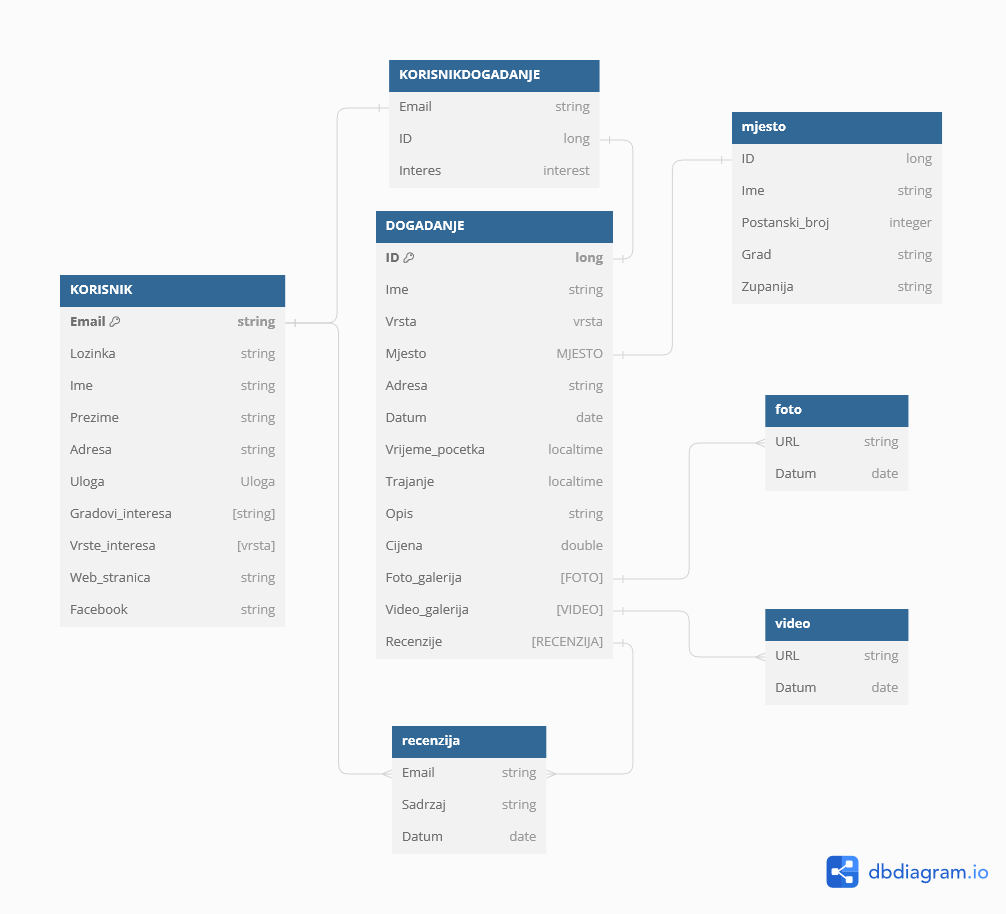
\includegraphics[width=\textwidth]{slike/Dijagram_baza.PNG} %veličina u odnosu na širinu linije
			\caption{Dijagram baze podataka}
			\label{fig:DB} %label mora biti drugaciji za svaku sliku
		\end{figure}
			\eject
			
			
		\section{Dijagram razreda}
		
		
		\begin{comment}
			\textit{Potrebno je priložiti dijagram razreda s pripadajućim opisom. Zbog preglednosti je moguće dijagram razlomiti na više njih, ali moraju biti grupirani prema sličnim razinama apstrakcije i srodnim funkcionalnostima.}\\
			
			\textbf{\textit{dio 1. revizije}}\\
			
			\textit{Prilikom prve predaje projekta, potrebno je priložiti potpuno razrađen dijagram razreda vezan uz \textbf{generičku funkcionalnost} sustava. Ostale funkcionalnosti trebaju biti idejno razrađene u dijagramu sa sljedećim komponentama: nazivi razreda, nazivi metoda i vrste pristupa metodama (npr. javni, zaštićeni), nazivi atributa razreda, veze i odnosi između razreda.}\\
			
			\textbf{\textit{dio 2. revizije}}\\			
			
			\textit{Prilikom druge predaje projekta dijagram razreda i opisi moraju odgovarati stvarnom stanju implementacije}
		\end{comment}
		
			Na slikama \ref{fig:DRC} i \ref{fig:DRM} prikazani su razredi koji pripadaju backend dijelu arhitekture aplikacije. Razredi prikazani na slici \ref{fig:DRC} nasljeđuju razred Controller i primarno služe za dohvaćanje i manipulaciju podataka u sustavu. Na slici \ref{fig:DRM} prikazan je dijagram koji preslikava strukturu baze podataka. Metode u tim razredima direktno komuniciraju s bazom podataka. Razred User predstavlja korisnika čiju vrstu određuje enumeracija Role. Ovisno o vrijednosti te enumeracije, može se raditi o posjetitelju, administratoru ili organizatoru. Razred Event predstavlja objavljeno događanje koje je vrste određene vrijednosti enumeracije EventType. Razred Event kao atribute sadrži listu objekata razreda Photo i listu objekata razreda Video. Dva navedena razreda predstavljaju redom fotografije i videozapise događanja. Razred Event također sadrži listu objekata razreda EventUser. Razred EventUser predstavlja oznaku kojom je korisnik označio određeni događaj. Taj razred dakle povezuje korisnika s nekom vrijednosti iz enumeracije Interest. Razred Event također sadrži listu objekata razreda Review koji predstavlja recenzije koje su korisnici ostavili za određeno događanje.
		
		
		\begin{figure}[H]
			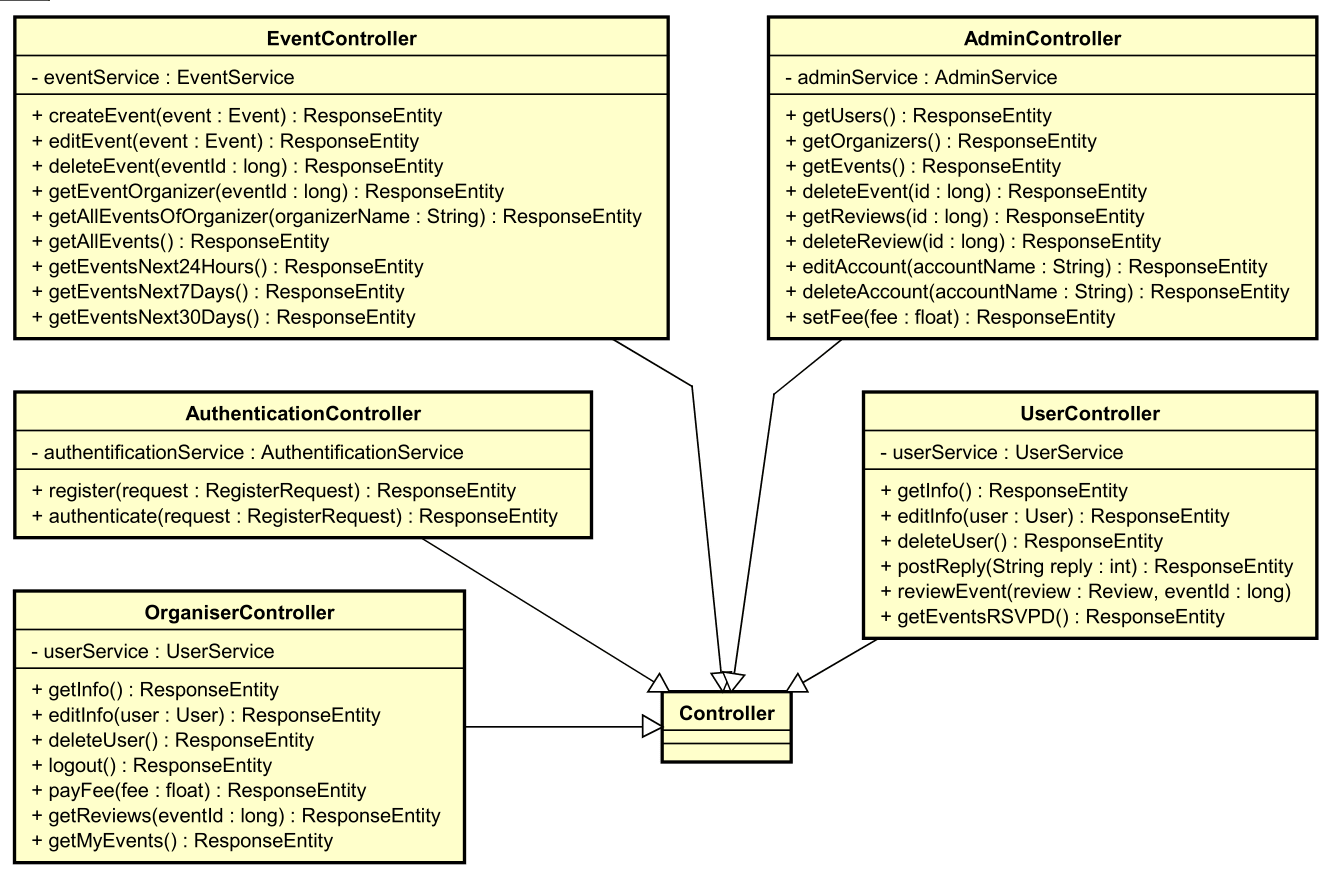
\includegraphics[width=\textwidth]{slike/DRC-1.PNG} %veličina u odnosu na širinu linije
			\caption{Dijagram razreda - Controllers}
			\label{fig:DRC} %label mora biti drugaciji za svaku sliku
		\end{figure}
			
			
		\begin{figure}[H]
			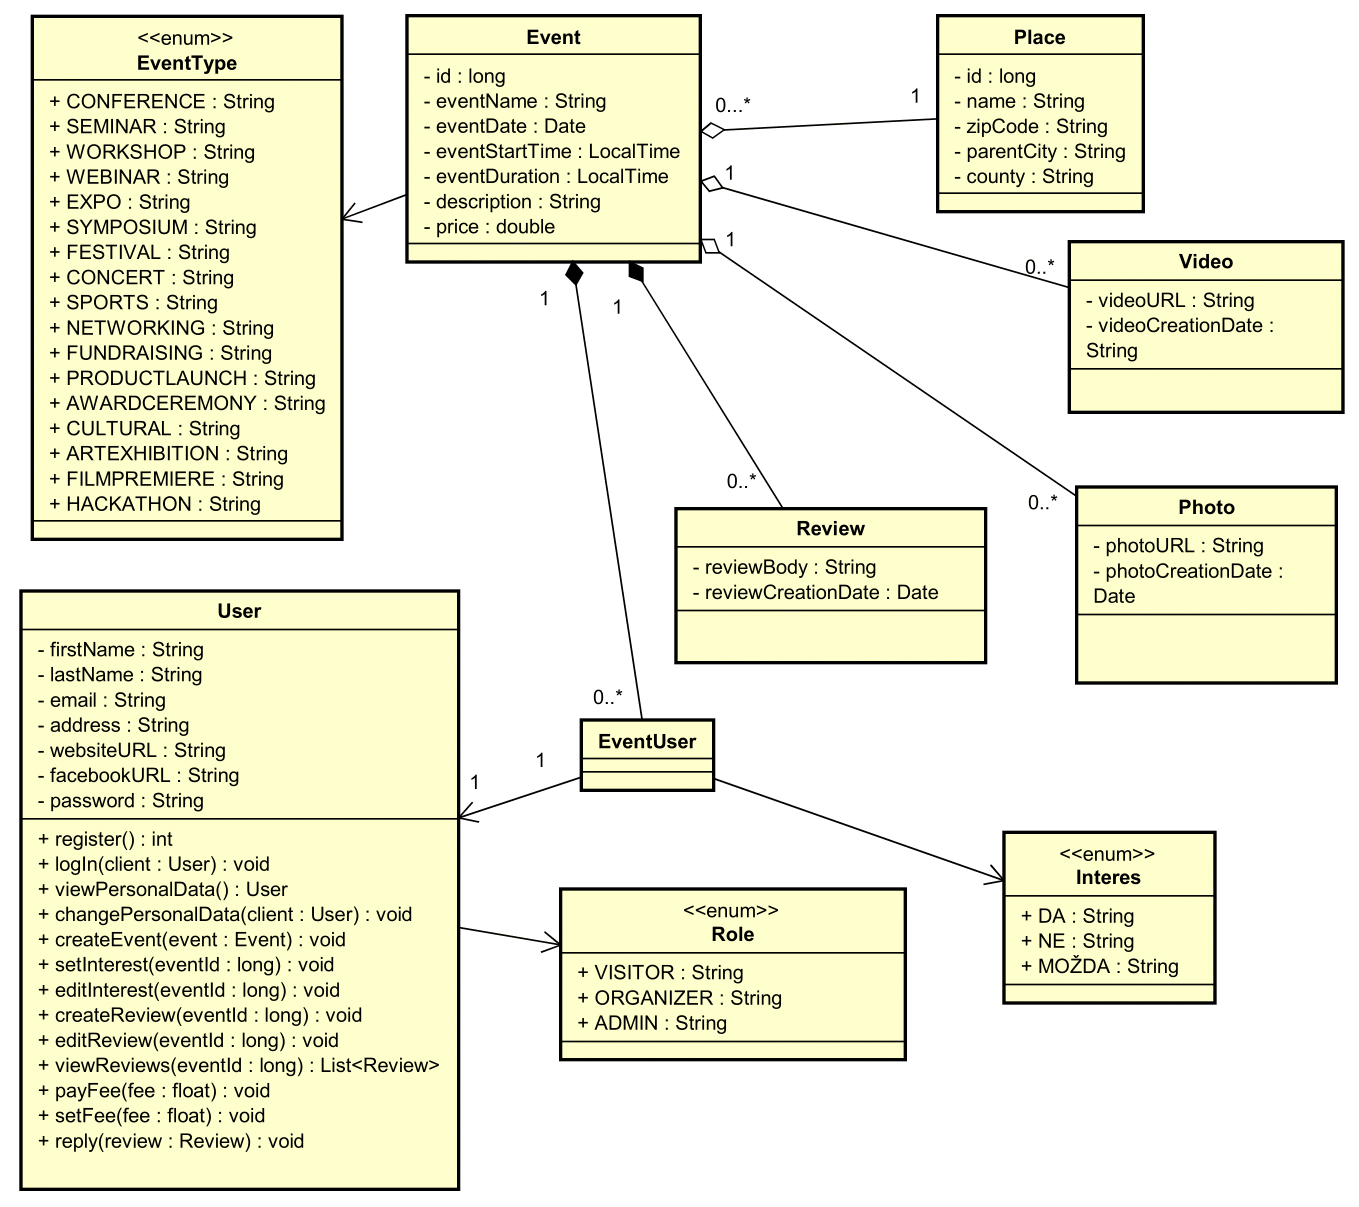
\includegraphics[width=\textwidth]{slike/DRM-1.PNG} %veličina u odnosu na širinu linije
			\caption{Dijagram razreda - Models}
			\label{fig:DRM} %label mora biti drugaciji za svaku sliku
		\end{figure}
			
			
			\eject
		
		\section{Dijagram stanja}
			
			\begin{comment}
			\textbf{\textit{dio 2. revizije}}\\
			
			\textit{Potrebno je priložiti dijagram stanja i opisati ga. Dovoljan je jedan dijagram stanja koji prikazuje \textbf{značajan dio funkcionalnosti} sustava. Na primjer, stanja korisničkog sučelja i tijek korištenja neke ključne funkcionalnosti jesu značajan dio sustava, a registracija i prijava nisu. }
			\end{comment}
			
			Dijagram stanja prikazuje stanja objekta te prijelaze iz jednog stanja u drugo temeljene na dogadajima. Slika \ref{fig:DSP} prikazuje dijagram stanja prijavljenog posjetitelja. Nakon prijave posjetitelju se na početnoj stranici prikazuje lista budućih događanja. Odabere li posjetitelj određeno događanje bit će mu ponuđene opcije da pročita više o događanju, označi dolaznost na događanje te da pogleda profil organizatora. Ako posjetitelj odabere pogledati profil organizatora otvoriti će mu se stranicu u kojoj će moći vidjeti recenzije ostaljene na neka događanja organizatora, buduća i prošla događanja te podatke o samom organizatoru. Ako posjetitelj želi pregledati svoj profil to će moći napraviti tako da odabere "Profil". Na toj će stranici moći pogledati i urediti svoje podatke, obrisati svoj račun, promjeniti interes za svoja buduća događanja, ostaviti osvrt na događanje na kojem je bio te urediti ili obrisati recenziju koju je već napisao.
			
			\begin{figure}[H]
			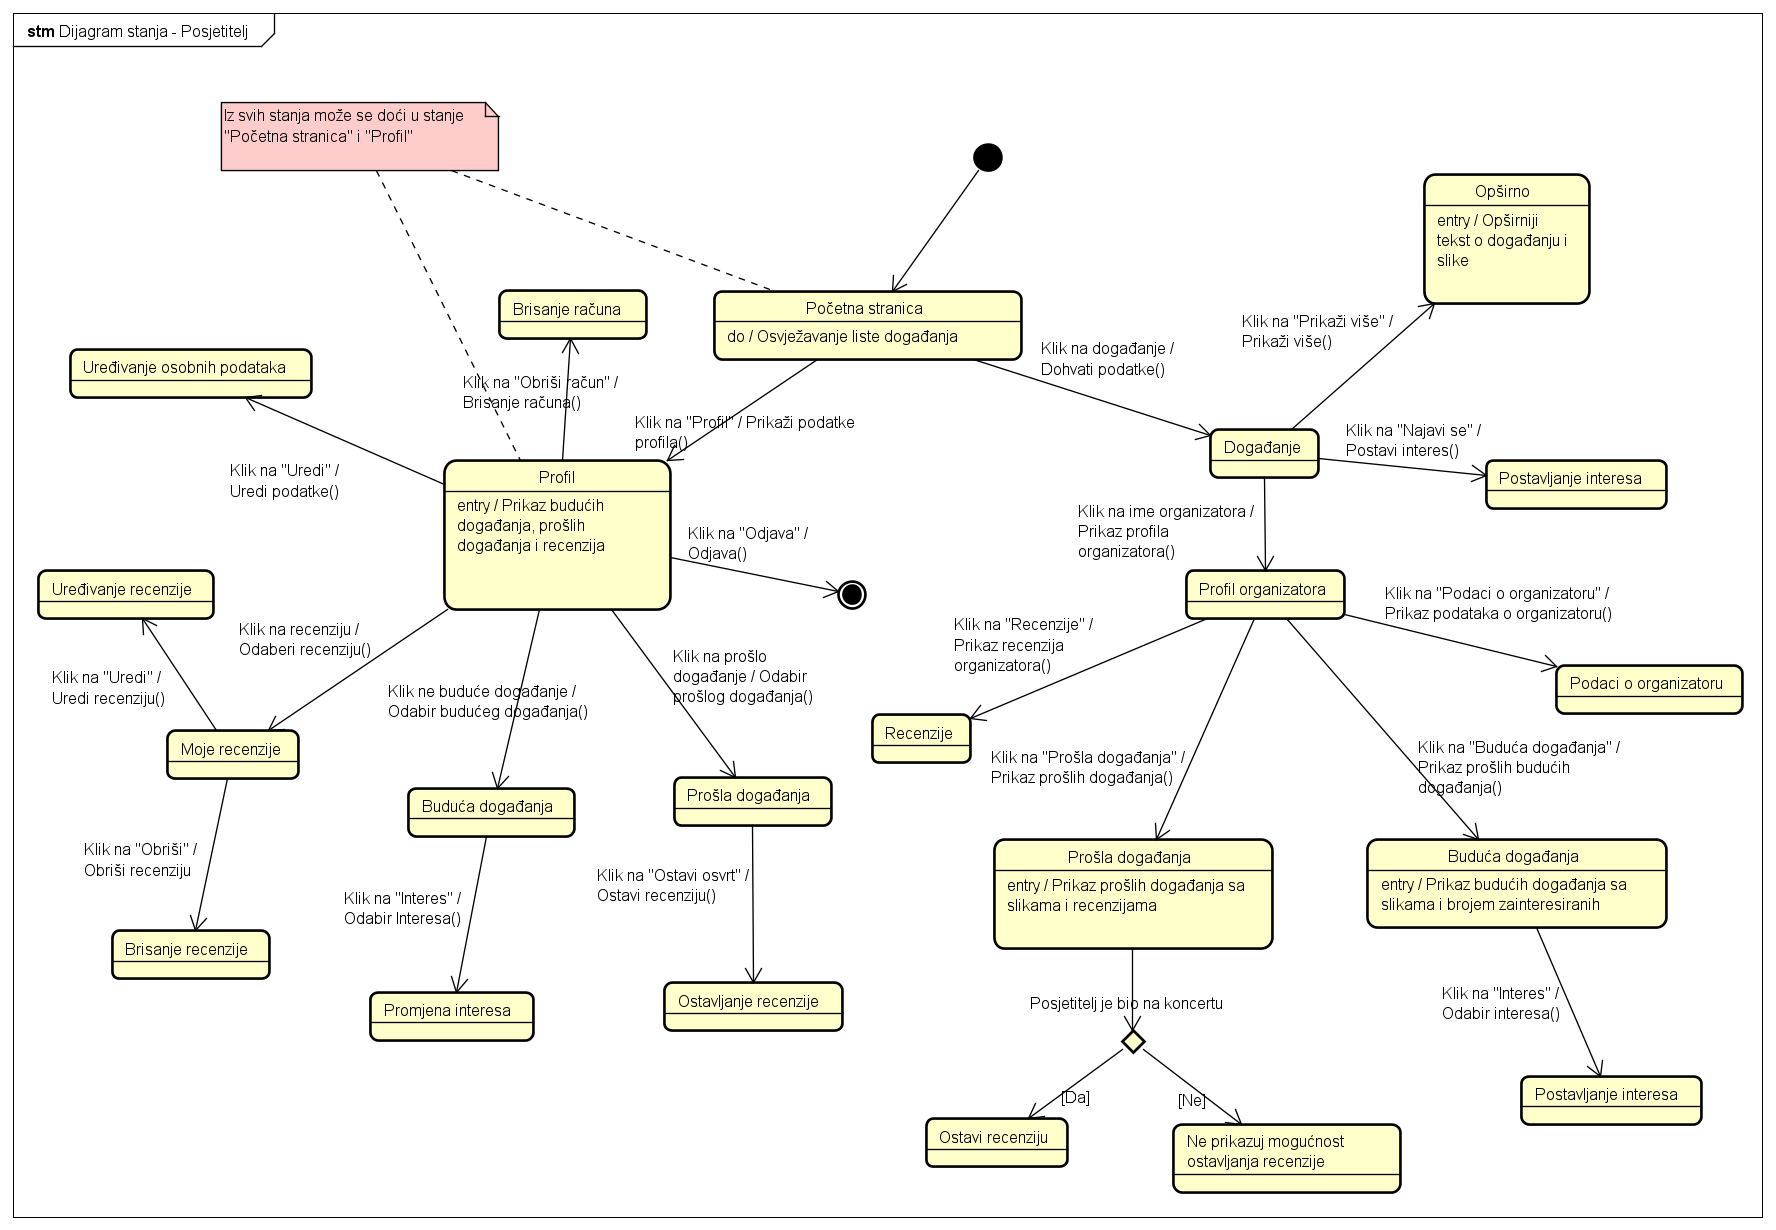
\includegraphics[width=\textwidth]{slike/Dijagram stanja - Posjetitelj.PNG} %veličina u odnosu na širinu linije
			\caption{Dijagram stanja - Posjetitelj}
			\label{fig:DSP} %label mora biti drugaciji za svaku sliku
		\end{figure}
			
			
			\eject 
		
		\section{Dijagram aktivnosti}
		
			Dijagram aktivnosti primjenjuje se za opis modela toka upravljanja ili toka podataka. Kao i kod sekvencijskog dijagrama kod dijagrama aktivnosti poseban naglasak ima redosljed kojim se aktivnosti isvršavaju. Zbog manjka kompleksnosti sustava u nastavku se nalaze dva dijagama aktivnosti. Prvi dijagram (\ref{fig:DAPZ}) prikazuje operacije sustava potrebne za postavljanje interesa na određeni događaj koji se još nije dogodio. Drugi dijagram (\ref{fig:DAOR}) prikazuje što se sve mora dogoditi da bi posjetitelj uspješno ostavio recenziju na događaj koji se već dogodio. 
			
			\begin{figure}[H]
			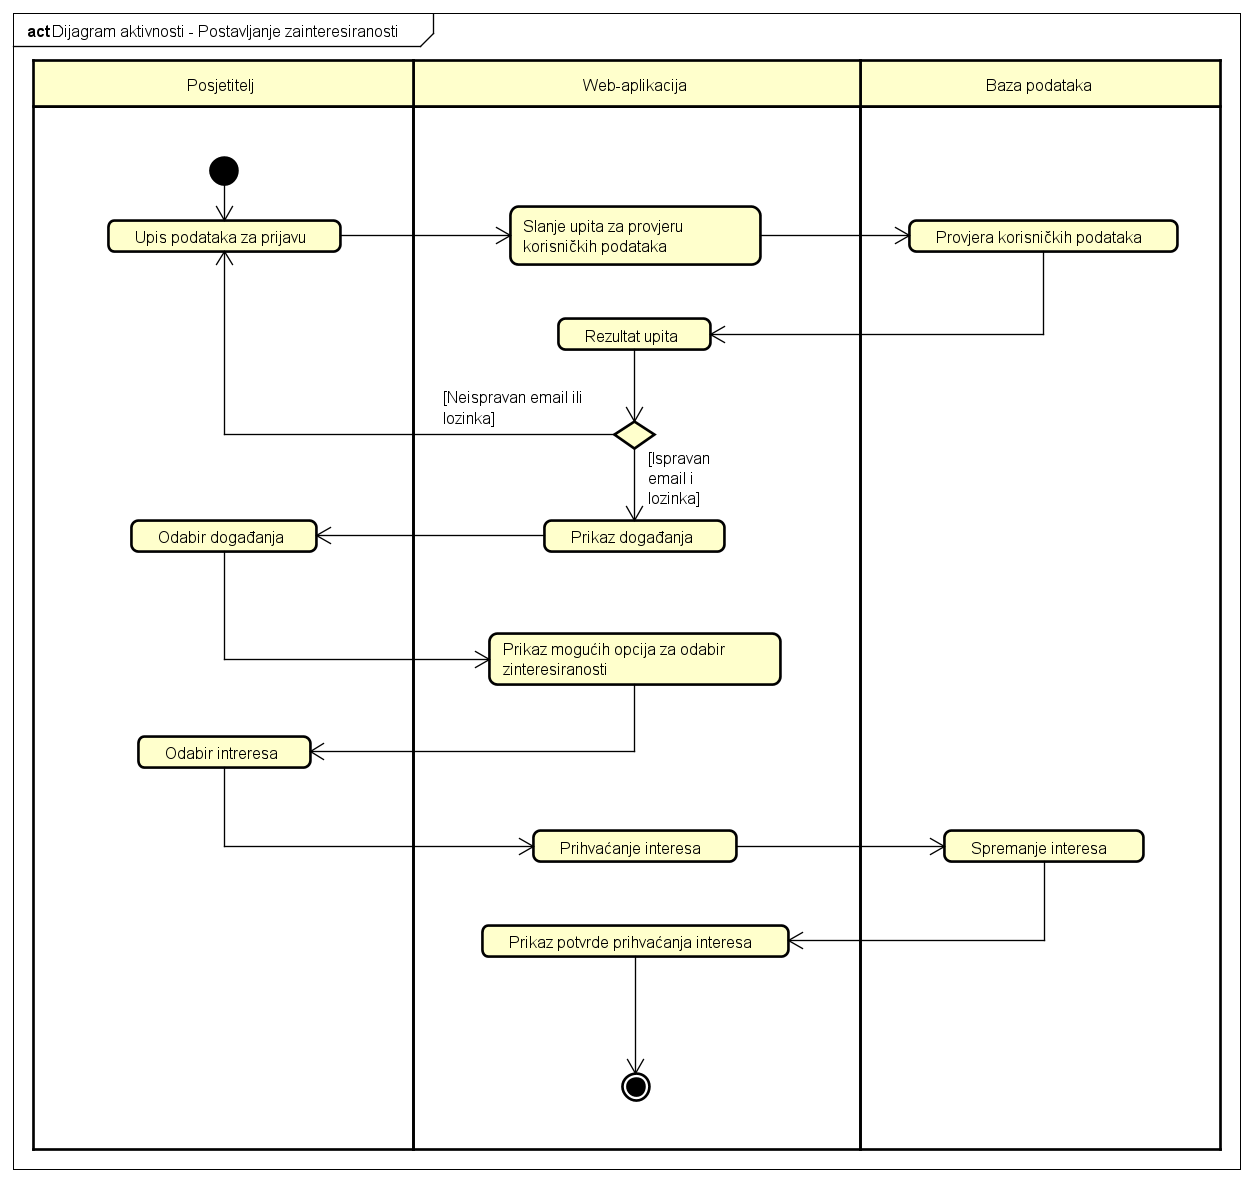
\includegraphics[width=\textwidth]{slike/Dijagram Aktivnosti - PZ.PNG} %veličina u odnosu na širinu linije
			\caption{Dijagram aktivnosti - Postavljanje zainteresiranosti}
			\label{fig:DAPZ} %label mora biti drugaciji za svaku sliku
		\end{figure}	
		
		\begin{figure}[H]
			\includegraphics[width=\textwidth]{slike/Dijagram Aktivnosti - OR.PNG} %veličina u odnosu na širinu linije
			\caption{Dijagram aktivnosti - Ostavljanje recenzije}
			\label{fig:DAOR} %label mora biti drugaciji za svaku sliku
		\end{figure}			
			
			\eject
		\section{Dijagram komponenti}
		
			\textbf{\textit{dio 2. revizije}}\\
		
			 \textit{Potrebno je priložiti dijagram komponenti s pripadajućim opisom. Dijagram komponenti treba prikazivati strukturu cijele aplikacije.}
	\chapter{Implementacija i korisničko sučelje}
		
		
		\section{Korištene tehnologije i alati}
		
			Za komunikaciju u timu korištene su aplikacije WhatsApp\footnote{\url{https://www.whatsapp.com/}} i Discord\footnote{\url{https://discord.com/}}. UML dijagrami izrađeni su pomoću alata Astah UML\footnote{\url{https://astah.net/products/astah-uml/}}, a zajedno s ostalim materijalima i informacijama u dokumentaciju su uneseni pomoću alata za uređivanje LaTeX dokumenata koji se zove Texmaker\footnote{\url{https://www.xm1math.net/texmaker/}} i beplatne verzije online alata iste vrste Overleaf\footnote{\url{https://www.overleaf.com/}}. Kao sustav za upravljanje izvornim kodom korišten je Git\footnote{\url{https://git-scm.com/}}, a udaljeni repozitorij nalazio se na web platformi GitHub\footnote{\url{https://github.com/}}. 

Kao razvojno okruženje korišteni su Visual Studio Code\footnote{\url{https://code.visualstudio.com/}}, uređivač koda kojie je razvijen od strane kompanije Microsoft za operacijske sustave Windows, Linux i macOS, i IntelliJ IDEA\footnote{\url{https://www.jetbrains.com/idea/}}, integrirano razvojno okruženje (IDE) razvijeno od strane kompanije JetBrains. Backend je realiziran pomoću radnog okvira Node.js\footnote{\url{https://nodejs.org/}} koji omogućuje korištenje jezika JavaScript\footnote{\url{https://www.javascript.com/}} na serverskoj strani aplikacije. API je pisan u jeziku Java\footnote{\url{https://www.java.com/}} uz korištenje radnog okvira Java Spring Boot\footnote{\url{https://spring.io/projects/spring-boot/}} koji ima ugrađenu podršku za zadatke poput upravljanja konfiguracijom, pristupa podatcima u bazi podataka i intergracije sigurnosti u aplikaciju. Aplikacija pristupa MongoDB\footnote{\url{https://www.mongodb.com/}} bazi podataka za čiji je lakši pregled korišten alat MongoDB Compass\footnote{\url{https://www.mongodb.com/products/tools/compass}}. Frontend je raliziran pomoću biblioteke React\footnote{\url{https://react.dev/}}, također poznate kao React.js ili ReactJS, koja omogućuje pisanje HTML koda u JavaScript datotekama što, skupa s modularnom arhitekturom i komponentama koje pruža biblioteka, čini jednostavnim dinamičko generiranje korisničkih sučelja. Za lakše stvaranje nekih komponenti korisnočkog sučelja korišten je radni okvir Bootstrap\footnote{\url{https://getbootstrap.com/}} koji pruža HTML, CSS i JavaScript kod često potrebnih dijelova aplikacije.

Za testiranje API-ja korišten je alat Postman\footnote{\url{https://www.postman.com/}} koji omogućuje slanje različitih vrsta zahtjeva na server. Aplikacija je testirana pomoću alata Selenium WebDriver\footnote{\url{https://www.selenium.dev/documentation/webdriver/}} i JUnit\footnote{\url{https://junit.org/}}, koji omogućuju automatizaciju testiranja web aplikacija pomoću programskog sučelja. Interakcija Selenium WebDrivera s Google Chrome pretraživačem ostavrena alatom ChromeDriver\footnote{\url{https://chromedriver.chromium.org/}}.
			\eject 
		
	
		\section{Ispitivanje programskog rješenja}
			
			\subsection{Ispitivanje komponenti}
			\noindent \textbf{Testni slučaj 1: Provjera addEvent funkcije u Event servisu}
						\begin{itemize}
	
						\item[] \textbf{Ulaz: }
						\begin{packed_enum}
							\item Inicijalizacija događanja
							\item Dodavanje imena "Test Event" događanju 
							\item Pokretanje funkcije \textit{addEvent}
							\item Provjera podudaranja testnog imena s imenom novo nastalog događanja u bazi 
						
						\end{packed_enum}
						\item[] \textbf{Očekivani rezultat: }
						\begin{packed_enum}
							\item Imena će se podudarati
						
						\end{packed_enum}
						\item[] \textbf{Rezultat: }
						\begin{packed_enum}
							\item  Imena se podudaraju
						
						\end{packed_enum}
						\end{itemize}
						
						\begin{figure}[H]
							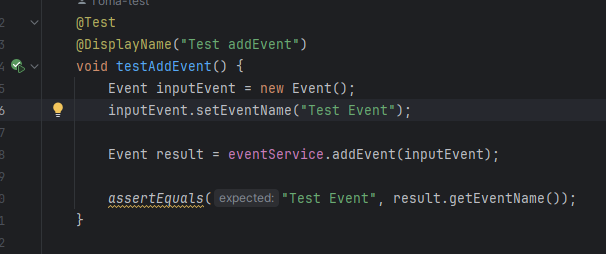
\includegraphics[width=\textwidth]{slike/IKTest1.PNG} %veličina u odnosu na širinu linije
							\caption{Prvi testni slučaj - addEvent}
							\label{fig:IKT1} %label mora biti drugaciji za svaku sliku
						\end{figure}
						\eject
						
						
						
			\noindent \textbf{Testni slučaj 2: Provjera editEvent funkcije u Event servisu}
						\begin{itemize}
	
						\item[] \textbf{Ulaz: }
						\begin{packed_enum}
							\item Inicijalizacija događanja
							\item Dodavanje imena "Original Event Name" i ID-a događanju 
							\item Spremanje događanja pomoću funkcije \textit{addEvent}
							\item Zadavanje novog imena "Updated Event Name" događanju
							\item Pokretanje funkcije \textit{editEvent}
							\item Usporedba uređenog imena sa imenom događanja u bazi
						
						\end{packed_enum}
						\item[] \textbf{Očekivani rezultat: }
						\begin{packed_enum}
							\item Imena će se podudarati
						
						\end{packed_enum}
						\item[] \textbf{Rezultat: }
						\begin{packed_enum}
							\item Događanje ima novo ime koje se podudara "Updated Event Name"
						
						\end{packed_enum}
						\end{itemize}
						
						\begin{figure}[H]
							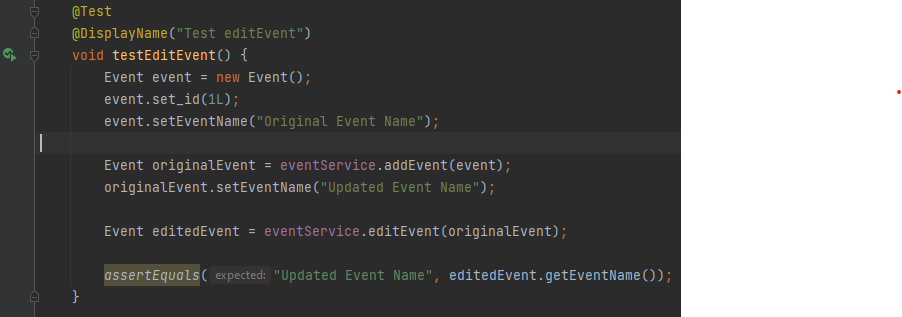
\includegraphics[width=\textwidth]{slike/IKTest2.PNG} %veličina u odnosu na širinu linije
							\caption{Drugi testni slučaj - editEvent}
							\label{fig:IKT2} %label mora biti drugaciji za svaku sliku
						\end{figure}
						\eject
						
						
						
			\noindent \textbf{Testni slučaj 3: Provjera getUserById funkcije u User servisu}
						\begin{itemize}
	
						\item[] \textbf{Ulaz: }
						\begin{packed_enum}
							\item Zadavanje ID-a za pronalaženje
							\item Dohvaća se korisnik s tim ID-em izravno iz baze
							\item Pokretanje funkcije \textit{getUserById} za zadani ID
							\item Usporedba dohvaćenog korisnika izravno iz baze i korisnika dohvaćenog preko funkcije \textit{getUserById}
						
						\end{packed_enum}
						\item[] \textbf{Očekivani rezultat: }
						\begin{packed_enum}
							\item Korisnici su jednaki
						
						\end{packed_enum}
						\item[] \textbf{Rezultat: }
						\begin{packed_enum}
							\item Dohvaćeni korisnici se podudaraju
						
						\end{packed_enum}
						\end{itemize}
						
						\begin{figure}[H]
							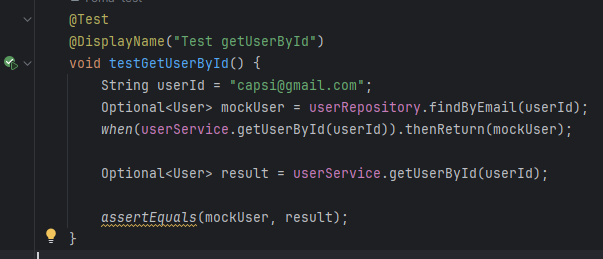
\includegraphics[width=\textwidth]{slike/IKTest3.PNG} %veličina u odnosu na širinu linije
							\caption{Treći testni slučaj - getUserById}
							\label{fig:IKT3} %label mora biti drugaciji za svaku sliku
						\end{figure}
						\eject
						
						
						
			\noindent \textbf{Testni slučaj 4: Provjera getUserById funkcije u User servisu (neuspješno)}
						\begin{itemize}
	
						\item[] \textbf{Ulaz: }
						\begin{packed_enum}
							\item Zadavanje ID-a za pronalaženje
							\item Dohvaća se korisnik s tim ID-em izravno iz baze
							\item Pokretanje funkcije \textit{getUserById} za zadani ID
							\item Usporedba dohvaćenog korisnika izravno iz baze i korisnika dohvaćenog preko funkcije \textit{getUserById}
						
						\end{packed_enum}
						\item[] \textbf{Očekivani rezultat: }
						\begin{packed_enum}
							\item Uspoređuju se dvije prezne vrijednosti jer takav korisnik ne postoji
						
						\end{packed_enum}
						\item[] \textbf{Rezultat: }
						\begin{packed_enum}
							\item Test prolazi jer su obje vraćene vrijednosti prazne
							
						
						\end{packed_enum}
						\end{itemize}
						
						\begin{figure}[H]
							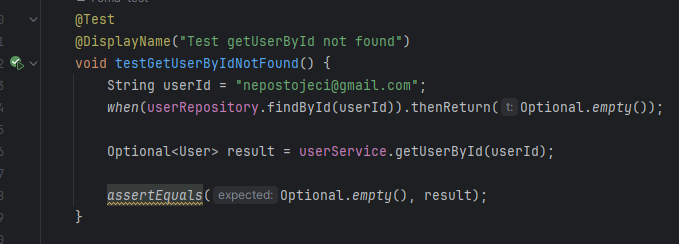
\includegraphics[width=\textwidth]{slike/IKTest4.PNG} %veličina u odnosu na širinu linije
							\caption{Četvrti testni slučaj - getUserById (nepostojeći)}
							\label{fig:IKT4} %label mora biti drugaciji za svaku sliku
						\end{figure}
						\eject
						
						
						
			\noindent \textbf{Testni slučaj 5: Provjera allEvents funkcije u Event servisu}
						\begin{itemize}
	
						\item[] \textbf{Ulaz: }
						\begin{packed_enum}
							\item Dohvaćanje svih događanja izravno iz baze
							\item Pozivanje funkcije \textit{allEvents}
							\item Usporedba dohvaćenih događanja iz baze s dohvaćenim događanjima preko \textit{allEvents} funkcije
						
						\end{packed_enum}
						\item[] \textbf{Očekivani rezultat: }
						\begin{packed_enum}
							\item Dobivena događanja se podudaraju
						
						\end{packed_enum}
						\item[] \textbf{Rezultat: }
						\begin{packed_enum}
							\item Popisi događanja se podudaraju
							
						
						\end{packed_enum}
						\end{itemize}
						
						\begin{figure}[H]
							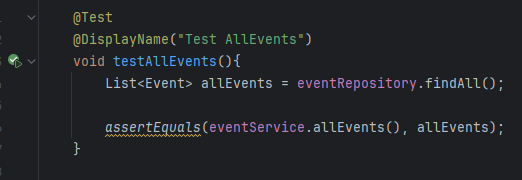
\includegraphics[width=\textwidth]{slike/IKTest5.PNG} %veličina u odnosu na širinu linije
							\caption{Peti testni slučaj - allEvents}
							\label{fig:IKT5} %label mora biti drugaciji za svaku sliku
						\end{figure}
						\eject
						
						
						
			\noindent \textbf{Testni slučaj 6: Provjera getEventById funkcije u Event servisu}
						\begin{itemize}
	
						\item[] \textbf{Ulaz: }
						\begin{packed_enum}
							\item Dohvaćanje događanja preko ID-a izravno iz baze
							\item Pozivanje funkcije \textit{getEventById} za isti ID
							\item Usporedba dohvaćenog događanja iz baze s dohvaćenim događanjem preko \textit{getEventById} funkcije
						
						\end{packed_enum}
						\item[] \textbf{Očekivani rezultat: }
						\begin{packed_enum}
							\item Dobivena događanja se podudaraju
						
						\end{packed_enum}
						\item[] \textbf{Rezultat: }
						\begin{packed_enum}
							\item Događanja se podudaraju
							
						
						\end{packed_enum}
						\end{itemize}
						
						\begin{figure}[H]
							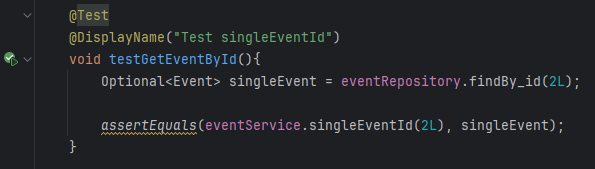
\includegraphics[width=\textwidth]{slike/IKTest6.PNG} %veličina u odnosu na širinu linije
							\caption{Šesti testni slučaj - getUserById}
							\label{fig:IKT6} %label mora biti drugaciji za svaku sliku
						\end{figure}
						\eject
						
				\noindent \textbf{Uspješnost testova - Ispitivanje komponenata}
						\begin{figure}[H]
							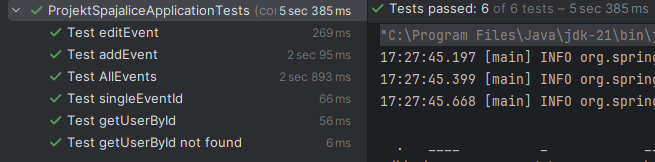
\includegraphics[width=\textwidth]{slike/IKTestovi.PNG} %veličina u odnosu na širinu linije
							\caption{Svi testovi komponenti}
							\label{fig:IKTS} %label mora biti drugaciji za svaku sliku
						\end{figure}
						\eject
						
						
			
			
			
			\subsection{Ispitivanje sustava}
			
				\noindent \textbf{Testni slučaj 1: Provjera \textit{Login} funkcionalnosti (UC3)}
						\begin{itemize}
	
						\item[] \textbf{Ulaz: }
						\begin{packed_enum}
							\item Otvaranje login stranice
							\item Upisivanje podataka za prijavu
							\item Unos podataka u aplikaciju
						
						\end{packed_enum}
						\item[] \textbf{Očekivani rezultat: }
						\begin{packed_enum}
							\item Dobiven novi url kojim se dolazi na prijavljeno sučelje
						
						\end{packed_enum}
						\item[] \textbf{Rezultat: }
						\begin{packed_enum}
							\item Test uspješan
							
						
						\end{packed_enum}
						\end{itemize}
						
						\begin{figure}[H]
							\includegraphics[width=\textwidth]{slike/IsTest1.PNG} %veličina u odnosu na širinu linije
							\caption{Prvi testni slučaj - Login}
							\label{fig:IST1} %label mora biti drugaciji za svaku sliku
						\end{figure}
						\eject
						
						
						
				\noindent \textbf{Testni slučaj 2: Provjera \textit{Login} funkcionalnosti (pogrešni podatci) (UC3)}
						\begin{itemize}
	
						\item[] \textbf{Ulaz: }
						\begin{packed_enum}
							\item Otvaranje login stranice
							\item Upisivanje podataka za prijavu
							\item Unos podataka u aplikaciju
						
						\end{packed_enum}
						\item[] \textbf{Očekivani rezultat: }
						\begin{packed_enum}
							\item Nije dobiven traženi url i javlja se poruka o pogrešno unesenim podatcima
						
						\end{packed_enum}
						\item[] \textbf{Rezultat: }
						\begin{packed_enum}
							\item Test uspješan
							
						
						\end{packed_enum}
						\end{itemize}
						
						\begin{figure}[H]
							\includegraphics[width=\textwidth]{slike/IsTest2.PNG} %veličina u odnosu na širinu linije
							\caption{Drugi testni slučaj - Login (pogrešni podatci)}
							\label{fig:IST2} %label mora biti drugaciji za svaku sliku
						\end{figure}
						\eject
						
						
						
				\noindent \textbf{Testni slučaj 3: Provjera funkcionalnosti kreiranja događanja (UC14)}
						\begin{itemize}
	
						\item[] \textbf{Ulaz: }
						\begin{packed_enum}
							\item Otvaranje login stranice
							\item Prijava
							\item Otvaranje padajućeg izbornika 
							\item Odabir opcije stvaranja događanja
							\item Upisivanje podataka o događanju
							\item Unos podataka u aplikaciju
							
						
						\end{packed_enum}
						\item[] \textbf{Očekivani rezultat: }
						\begin{packed_enum}
							\item Otvaranje \textit{pop up} prozora s potvrdom o stvaranju događanja
						
						\end{packed_enum}
						\item[] \textbf{Rezultat: }
						\begin{packed_enum}
							\item Test uspješan
							
						
						\end{packed_enum}
						\end{itemize}
						
						\begin{figure}[H]
							\includegraphics[width=\textwidth]{slike/IsTest3.PNG} %veličina u odnosu na širinu linije
							\caption{Treći testni slučaj - Kreiranje događanja}
							\label{fig:IST3} %label mora biti drugaciji za svaku sliku
						\end{figure}
						\eject
						
						
						
				\noindent \textbf{Testni slučaj 4: Provjera funkcionalnosti promjene lozinke (UC5)}
						\begin{itemize}
	
						\item[] \textbf{Ulaz: }
						\begin{packed_enum}
							\item Otvaranje login stranice
							\item Prijava
							\item Otvaranje padajućeg izbornika 
							\item Odabir opcije pregleda profila
							\item Klika na gumb za promjenu lozinke
							\item Upisivanje stare i nove lozinke
							\item Unos podataka u aplikaciju
							
						
						\end{packed_enum}
						\item[] \textbf{Očekivani rezultat: }
						\begin{packed_enum}
							\item Otvaranje \textit{pop up} prozora s potvrdom o promjeni lozinke
						
						\end{packed_enum}
						\item[] \textbf{Rezultat: }
						\begin{packed_enum}
							\item Test uspješan
							
						
						\end{packed_enum}
						\end{itemize}
						
						\begin{figure}[H]
							\includegraphics[width=\textwidth]{slike/IsTest4.PNG} %veličina u odnosu na širinu linije
							\caption{Četvrti testni slučaj - Promjena lozinke}
							\label{fig:IST4} %label mora biti drugaciji za svaku sliku
						\end{figure}
						\eject
						
						
						
				\noindent \textbf{Testni slučaj 5: Provjera funkcionalnosti promjene prikaza profila}
						\begin{itemize}
	
						\item[] \textbf{Ulaz: }
						\begin{packed_enum}
							\item Otvaranje login stranice
							\item Prijava
							\item Otvaranje padajućeg izbornika 
							\item Odabir opcije pregleda profila
							\item Klik na gumb za otvaranje prikaza javnog profila
							
						
						\end{packed_enum}
						\item[] \textbf{Očekivani rezultat: }
						\begin{packed_enum}
							\item Dobiven novi url kojim se dolazi na prikaz javnog profila
						
						\end{packed_enum}
						\item[] \textbf{Rezultat: }
						\begin{packed_enum}
							\item Test uspješan
							
						
						\end{packed_enum}
						\end{itemize}
						
						\begin{figure}[H]
							\includegraphics[width=\textwidth]{slike/IsTest5.PNG} %veličina u odnosu na širinu linije
							\caption{Peti testni slučaj - Otvaranje prikaza javnog profila}
							\label{fig:IST5} %label mora biti drugaciji za svaku sliku
						\end{figure}
						\eject
						
						
						\noindent \textbf{Uspješnost testova - Ispitivanje sustava}
						\begin{figure}[H]
							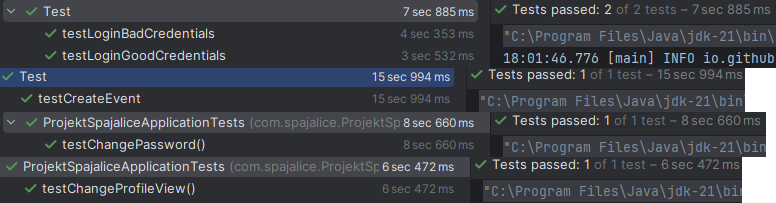
\includegraphics[width=\textwidth]{slike/ISTestovi.PNG} %veličina u odnosu na širinu linije
							\caption{Svi testovi sustava}
							\label{fig:ISTS} %label mora biti drugaciji za svaku sliku
						\end{figure}
						\eject
				
			
		
		
		\section{Dijagram razmještaja}
		Dijagram razmještaja (\ref{fig:DR}) prikazuje fizičku arhitekturu i konfiguraciju razmještaja programskog sustava. Poslužiteljsko računalo sadrži web poslužitelj na kojem je web aplikcaija i poslužitelj baze podataka koji omogućava pristup bazi. Klijent se na sustav spaja pomoću vlastitog osobnog računala koje uspostavlja komunikaciju preko HTTP protokola s poslužiteljskim računalom.  
			
			 \begin{figure}[H]
			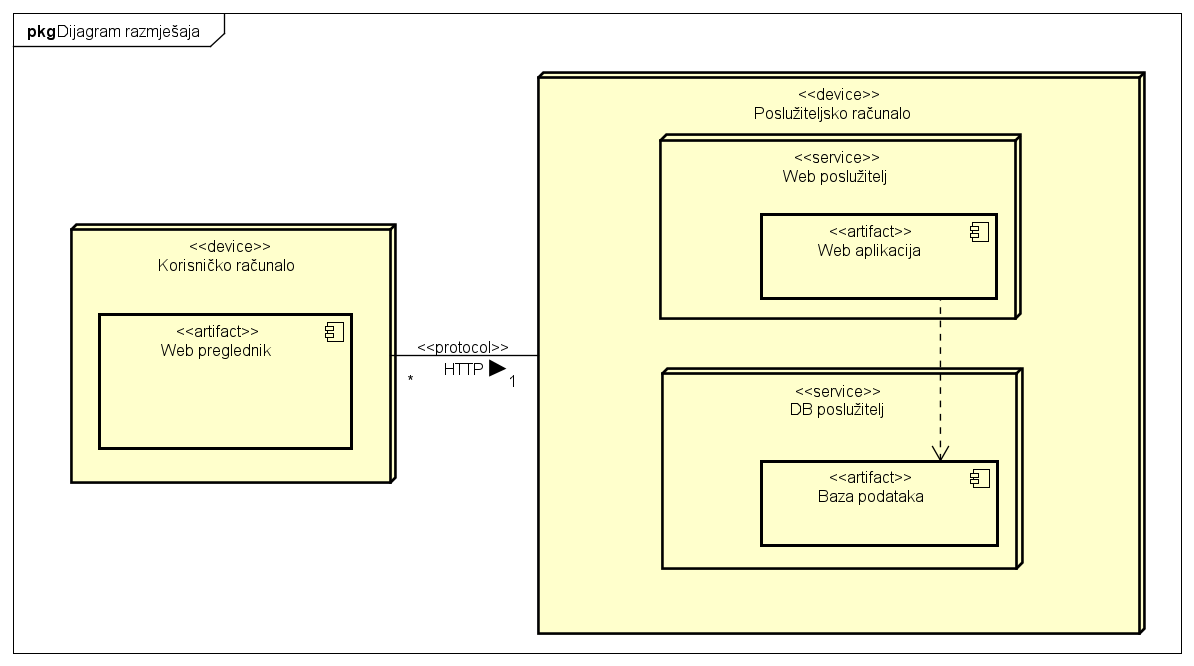
\includegraphics[width=\textwidth]{slike/Dijagram razmjestaja.PNG} %veličina u odnosu na širinu linije
			\caption{Dijagram razmještaja}
			\label{fig:DR} %label mora biti drugaciji za svaku sliku
		\end{figure}
			\eject 
		
		\section{Upute za puštanje u pogon}
		
			\textbf{\textit{dio 2. revizije}}\\
		
			 \textit{U ovom poglavlju potrebno je dati upute za puštanje u pogon (engl. deployment) ostvarene aplikacije. Na primjer, za web aplikacije, opisati postupak kojim se od izvornog kôda dolazi do potpuno postavljene baze podataka i poslužitelja koji odgovara na upite korisnika. Za mobilnu aplikaciju, postupak kojim se aplikacija izgradi, te postavi na neku od trgovina. Za stolnu (engl. desktop) aplikaciju, postupak kojim se aplikacija instalira na računalo. Ukoliko mobilne i stolne aplikacije komuniciraju s poslužiteljem i/ili bazom podataka, opisati i postupak njihovog postavljanja. Pri izradi uputa preporučuje se \textbf{naglasiti korake instalacije uporabom natuknica} te koristiti što je više moguće \textbf{slike ekrana} (engl. screenshots) kako bi upute bile jasne i jednostavne za slijediti.}
			
			
			 \textit{Dovršenu aplikaciju potrebno je pokrenuti na javno dostupnom poslužitelju. Studentima se preporuča korištenje neke od sljedećih besplatnih usluga: \href{https://aws.amazon.com/}{Amazon AWS}, \href{https://azure.microsoft.com/en-us/}{Microsoft Azure} ili \href{https://www.heroku.com/}{Heroku}. Mobilne aplikacije trebaju biti objavljene na F-Droid, Google Play ili Amazon App trgovini.}
			
			
			\eject 
	\chapter{Zaključak i budući rad}
		
		Nakon 14 tjedana izrade aplikacije za objavu i traženje događanja u blizini ostvaren je zadani cilj. Većina funkcionalnosti je implementirana radi ispravno. Tim se pokazao izrazito plodonosan i usklađen. Prema zadanim kontrolnim točkama faze rada se mogu podjeliti u dvije cjeline. 
		Prva faza poslužila je za dogovor oko podjele poslova i zaključak kako će se u njoj veći fokus staviti na dokumentaciju. Iz tog je rezloga tim podjeljen u tri manja podtima: backend, frontend i dokumentaciju. Definirani podtimovi nisu garantirali da će se njihovi članovi baviti samo područjem tog podtima već je donesena odluka kako će si članovi različitih podtimova međusobno pomagati kako bi svi iskusili svaki dio projekta. Tako je u ovoj fazi podtim dokumentacije dobivao konstantne povratne informacije o dogovorima oko arhitektura koje će se koristiti i na koji način. Kako bi se najkvalitetnije dogovorili svi su članovi bili prisutni na gotovo svim sastancima. 
		U drugoj je fazi stavljen naglasak na programskom rješenju te su se svi članovi aktivnije počeli baviti razvijanjem sustava u praksi. Kako bi svi znali što treba raditi poslužio im je plan iz dokumentacije sastavljen u prvoj fazi. U ovoj je fazi došlo do promjene načina komunikacije, projekt više nije zahtjevao prisutnost svih članova od jednom već bi se članovi međusobno savjetovali kako nebi prelazili preko tuđih rješenja. Dokumentacija se u ovoj fazi radila paralelno s razvojem programskog rješenja jer su određeni dijelovi zahtjevali testiranje samog rješenja. 
		Komunikacija se pokazala kao ključan faktor u uspješnosti i efikasnosti izrade projekta. Za uspješno uspostavljenu komunikacijeu treba dati posebne hvale voditelj grupe koji kvalitetno je podjelio zadatke i uvijek bio na usluzi kada je situacija to zahtjevala. Svi su članovi bili zainteresirani i odlučni u odluci da se projekt napravi na što bolji način. 
		Problem na koji su gotovo svi članovi naišli bio je manjak iskustva u korištenju odabranih alata. Manjak iskustva bio je vidljiv i u samom upravljanju projektom gdje je bilo potrebno vrijeme da svaki član ustanovi koja je točno njegova uloga u timu.
		Radi manjka vremena neke zahtjevnije funkcionalnosti nisu mogle biti implementirane no zadatak je gotovo u potpunosti obavljen. Među funkcionalnostima koje nisu implementiorane nalaze se pretplaćivanje na organizatora i objava videozapisa.
		Tim nije pokazivao naznake ne slaganja i loših odnosa međutim odluka o nastavku razvijanja aplikacije nije donesena. Tim je zaključio kako je sudjelovanje na projektu bilo vrijedno iskustvo za daljnji rad no kako sama ideja aplikacije nema primjenjivu namjenu koju bi članovi htijeli poduprijeti. Tim je kolektivno zadovoljan s postignutim razultatom i ne odbacuje mogućnost buduće suradnje.
		
	\chapter*{Popis literature}
		\addcontentsline{toc}{chapter}{Popis literature}
	 	
 		%\textbf{\textit{Kontinuirano osvježavanje}}
	
		%\textit{Popisati sve reference i literaturu koja je pomogla pri ostvarivanju projekta.}
		
		
		\begin{enumerate}
			
			
			\item  Programsko inženjerstvo, FER ZEMRIS, \url{http://www.fer.hr/predmet/proinz}
			
			\item  React, \url{https://react.dev/learn}
			
			\item  Spring,  Spring Boot,  \url{https://spring.io/projects/spring-boot}
			
			\item  MongoDB, \url{https://www.mongodb.com}
			
			\item  Geeks for geeks, MVC Framework, \url{https://www.geeksforgeeks.org/mvc-framework-introduction/?ref=gcse}
			
			\item  Astah Community, \url{http://astah.net/editions/uml-new}
			
			\item  Selenium WebDriver, \url{https://www.selenium.dev/documentation/webdriver/}
		\end{enumerate}
		
		 
	
	
	\begingroup
	\renewcommand*\listfigurename{Indeks slika i dijagrama}
	%\renewcommand*\listtablename{Indeks tablica}
	%\let\clearpage\relax
	\listoffigures
	%\vspace{10mm}
	%\listoftables
	\endgroup
	\addcontentsline{toc}{chapter}{Indeks slika i dijagrama}


	
	\eject 
		
	\chapter*{Dodatak: Prikaz aktivnosti grupe}
		\addcontentsline{toc}{chapter}{Dodatak: Prikaz aktivnosti grupe}
		
		\section*{Dnevnik sastajanja}
		
		\textbf{\textit{Kontinuirano osvježavanje}}\\
		
		 \textit{U ovom dijelu potrebno je redovito osvježavati dnevnik sastajanja prema predlošku.}
		
		\begin{packed_enum}
			\item  sastanak
			
			\item[] \begin{packed_item}
				\item Datum: 19. listopada 2023.
				\item Prisustvovali: Svi članovi
				\item Teme sastanka:
				\begin{packed_item}
					\item  sastanak s asistentom i demonstratorom
					\item  raspodjela poslova
					\item  biranje alata
				\end{packed_item}
			\end{packed_item}
			
			\item  sastanak
			\item[] \begin{packed_item}
				\item Datum: 23. listopada 2023.
				\item Prisustvovali: Svi članovi
				\item Teme sastanka:
				\begin{packed_item}
					\item  dodatan dogovor oko raspodjele poslova
					\item  konačan odabir alata
				\end{packed_item}
			\end{packed_item}
			
			\item  sastanak
			\item[] \begin{packed_item}
				\item Datum: 2. studenoga 2023.
				\item Prisustvovali: Mrvčić, Duvančić
				\item Teme sastanka:
				\begin{packed_item}
					\item  dogovor oko funkcionalnosti 
					\item  izrada dijagrama
				\end{packed_item}
			\end{packed_item}
			
			\item  sastanak
			\item[] \begin{packed_item}
				\item Datum: 3. studenogaa 2023.
				\item Prisustvovali: Svi članovi
				\item Teme sastanka:
				\begin{packed_item}
					\item  dogovor oko izgleda baze podataka
					\item dogovor oko obrazca uporabe
				\end{packed_item}
			\end{packed_item}
			
			\item  sastanak
			\item[] \begin{packed_item}
				\item Datum: 4. studenoga 2023.
				\item Prisustvovali: Duvančić, Mrvičić, Radošević
				\item Teme sastanka:
				\begin{packed_item}
					\item  razrada obrazaca uporabe
					\item  izrada dijagrama
				\end{packed_item}
			\end{packed_item}
			
			%
			
		\end{packed_enum}
		
		\eject
		\section*{Tablica aktivnosti}
		
			\textbf{\textit{Kontinuirano osvježavanje}}\\
			
			 \textit{Napomena: Doprinose u aktivnostima treba navesti u satima po članovima grupe po aktivnosti.}

			\begin{longtblr}[
					label=none,
				]{
					vlines,hlines,
					width = \textwidth,
					colspec={X[7, l]X[1, c]X[1, c]X[1, c]X[1, c]X[1, c]X[1, c]X[1, c]}, 
					vline{1} = {1}{text=\clap{}},
					hline{1} = {1}{text=\clap{}},
					rowhead = 1,
				} 
			
				\SetCell[c=1]{c}{} & \SetCell[c=1]{c}{\rotatebox{90}{\textbf{Ime Prezime voditelja}}} & \SetCell[c=1]{c}{\rotatebox{90}{\textbf{Ime Prezime }}} &	\SetCell[c=1]{c}{\rotatebox{90}{\textbf{Ime Prezime }}} & \SetCell[c=1]{c}{\rotatebox{90}{\textbf{Ime Prezime }}} &	\SetCell[c=1]{c}{\rotatebox{90}{\textbf{Ime Prezime }}} & \SetCell[c=1]{c}{\rotatebox{90}{\textbf{Ime Prezime }}} &	\SetCell[c=1]{c}{\rotatebox{90}{\textbf{Ime Prezime }}} \\  
				Upravljanje projektom 		&  &  &  &  &  &  & \\ 
				Opis projektnog zadatka 	&  &  &  &  &  &  & \\ 
				
				Funkcionalni zahtjevi       &  &  &  &  &  &  &  \\ 
				Opis pojedinih obrazaca 	&  &  &  &  &  &  &  \\ 
				Dijagram obrazaca 			&  &  &  &  &  &  &  \\ 
				Sekvencijski dijagrami 		&  &  &  &  &  &  &  \\ 
				Opis ostalih zahtjeva 		&  &  &  &  &  &  &  \\ 

				Arhitektura i dizajn sustava	 &  &  &  &  &  &  &  \\ 
				Baza podataka				&  &  &  &  &  &  &   \\ 
				Dijagram razreda 			&  &  &  &  &  &  &   \\ 
				Dijagram stanja				&  &  &  &  &  &  &  \\ 
				Dijagram aktivnosti 		&  &  &  &  &  &  &  \\ 
				Dijagram komponenti			&  &  &  &  &  &  &  \\ 
				Korištene tehnologije i alati 		&  &  &  &  &  &  &  \\ 
				Ispitivanje programskog rješenja 	&  &  &  &  &  &  &  \\ 
				Dijagram razmještaja			&  &  &  &  &  &  &  \\ 
				Upute za puštanje u pogon 		&  &  &  &  &  &  &  \\  
				Dnevnik sastajanja 			&  &  &  &  &  &  &  \\ 
				Zaključak i budući rad 		&  &  &  &  &  &  &  \\  
				Popis literature 			&  &  &  &  &  &  &  \\  
				&  &  &  &  &  &  &  \\ \hline 
				\textit{Dodatne stavke kako ste podijelili izradu aplikacije} 			&  &  &  &  &  &  &  \\ 
				\textit{npr. izrada početne stranice} 				&  &  &  &  &  &  &  \\  
				\textit{izrada baze podataka} 		 			&  &  &  &  &  &  & \\  
				\textit{spajanje s bazom podataka} 							&  &  &  &  &  &  &  \\ 
				\textit{back end} 							&  &  &  &  &  &  &  \\  
				 							&  &  &  &  &  &  &\\ 
			\end{longtblr}
					
					
		\eject
		\section*{Dijagrami pregleda promjena}
		
		\textbf{\textit{dio 2. revizije}}\\
		
		\textit{Prenijeti dijagram pregleda promjena nad datotekama projekta. Potrebno je na kraju projekta generirane grafove s gitlaba prenijeti u ovo poglavlje dokumentacije. Dijagrami za vlastiti projekt se mogu preuzeti s gitlab.com stranice, u izborniku Repository, pritiskom na stavku Contributors.}
		
	


\end{document} %naredbe i tekst nakon ove naredbe ne ulaze u izgrađen dokument 


